% !LW recipe = XeLaTeX once (current file)
\ifdefined\CourseRootDocument
\providecommand{\FinishStandaloneChapter}{}
\else
\documentclass[11pt,oneside,openany,UTF8,fontset=none]{ctexbook}
\def\StandaloneChapterNumber{7}
\def\StandaloneCourseSetup{\UseMacroIICourse}
% 单章/单附录构建前导区。
% 文档类声明保留在源文件中，便于 LaTeX Workshop 将当前文件识别为根文件；
% 本文件只补充共享前导区和正文环境。

% 单文件配方以源文件所在目录为工作目录；将项目根目录加入搜索路径，
% 因而文件名可包含空格和中文，也无需写入绝对的 iCloud 路径。
\makeatletter
\def\input@path{{../../}}
\makeatother
\newcommand{\ProjectRootPath}{../..}

% 全项目共享前导区：集中声明依赖顺序，整书与单章只引用这一处
% 用户可调文件位于 _config/，实现文件位于 _config/core/
% !TeX root = ../AdvMacroNote_Sun.tex
% Shared metadata plus the two course profiles used throughout the book.

\newcommand{\DocumentTitle}{Advanced Macroeconomics I \& II}
\newcommand{\DocumentVersion}{2nd edition}
\newcommand{\CourseTitle}{Advanced Macroeconomics I}
\newcommand{\CourseVolumeRoman}{I}
\newcommand{\CourseShortTitle}{Adv Macro I}
\newcommand{\CourseSubtitle}{(zh) Course notes based on the lectures of \CourseInstructor}
\newcommand{\CoursePartSubtitle}{Course notes based on the lectures of \CourseInstructor}
\newcommand{\CourseTerm}{Fall 2026}
\newcommand{\CourseInstructor}{Yinong TAN}
\newcommand{\CourseInstructorEmail}{}
\newcommand{\CourseCreditLabel}{Prepared by}
\newcommand{\CourseContributorLabel}{\CourseCreditLabel}
\newcommand{\CourseContributor}{Rongqing SUN}
\newcommand{\CourseContributorEmail}{econsunrq@outlook.com}
\newcommand{\CourseInstitution}{{\color{InstitutionMark}Xiamen University}}
\newcommand{\CourseAffiliation}{%
    SOE\hspace{0.5em}\(\boldsymbol{\times}\)\hspace{0.5em}%
    WISE\hspace{0.5em}\(\boldsymbol{\times}\)\hspace{0.5em}CHOW%
}
\newcommand{\CourseLevel}{Graduate Program}
% Short level label used only in the vertical page-edge metadata.
\newcommand{\CourseSideLevel}{Graduate}
\newcommand{\CoursePartAuthor}{\CourseContributor}
\newcommand{\CourseLicenseToken}{CC BY-NC 4.0}
\newcommand{\CoursePartDate}{\CourseCompileDate}
\newcommand{\CourseEmblem}{xmu-emblem.png}
\newcommand{\CourseUnitName}{Chapter}
% The shared cover treats each semester as its own reading unit.  Keeping
% these values separate avoids ambiguous slash-separated metadata.
\newcommand{\CoverSubtitle}{Lecture notes in Chinese}
\newcommand{\CoverFirstCourse}{Advanced Macroeconomics I}
\newcommand{\CoverFirstTerm}{Fall 2026}
\newcommand{\CoverFirstInstructor}{Yinong TAN}
\newcommand{\CoverFirstTopic}{Economic Growth}
\newcommand{\CoverSecondCourse}{Advanced Macroeconomics I}
\newcommand{\CoverSecondTerm}{Fall 2026}
\newcommand{\CoverSecondInstructor}{Yinong TAN}
\newcommand{\CoverSecondTopic}{Economic Fluctuation}
\newcommand{\CourseCompileDate}{%
    \ifcase\month\or
        January\or February\or March\or April\or May\or June\or
        July\or August\or September\or October\or November\or December%
    \fi~\number\day,~\number\year
}

\newcommand{\UseSharedCourseCover}{%
    \renewcommand{\CourseTitle}{\DocumentTitle}%
    \renewcommand{\CourseShortTitle}{Adv Macro I \& II}%
    \setcourseaccent{VolumeOneAccent}%
}
\newcommand{\UseMacroICourse}{%
    \renewcommand{\CourseTitle}{Advanced Macroeconomics I}%
    \renewcommand{\CourseShortTitle}{Adv Macro I}%
    \renewcommand{\CourseTerm}{Fall 2026}%
    \renewcommand{\CourseInstructor}{Yinong TAN}%
    \renewcommand{\CourseVolumeRoman}{I}%
    \setcourseaccent{VolumeOneAccent}%
}
\newcommand{\UseMacroIICourse}{%
    \renewcommand{\CourseTitle}{Advanced Macroeconomics I}%
    \renewcommand{\CourseShortTitle}{Adv Macro I}%
    \renewcommand{\CourseTerm}{Fall 2026}%
    \renewcommand{\CourseInstructor}{Yinong TAN}%
    \renewcommand{\CourseVolumeRoman}{I}%
    \setcourseaccent{VolumeTwoAccent}%
}

% Enable only after the notes contain active citation commands.
\newif\ifcoursebibliography
\coursebibliographyfalse

% !TeX root = ../AdvMacroNote_Sun.tex
% 主封面重要参数。没有单位的数值均表示 pt 字号。

% 顶部校徽模块：距页面顶部、校徽尺寸及图文水平距离。
% 文字以校徽的垂直中心定位，改变校徽尺寸时不需要重新调整文字高度。
\newcommand{\CoverIdentityTop}{22mm}
\newcommand{\CoverEmblemSize}{19mm}
\newcommand{\CoverEmblemTextGap}{6mm}
\newcommand{\CoverIdentityInstitutionSize}{14.5}
\newcommand{\CoverIdentityInstitutionLeading}{18}
\newcommand{\CoverIdentityAffiliationSize}{9.5}
\newcommand{\CoverIdentityAffiliationLeading}{12}
\newcommand{\CoverIdentityLevelSize}{10.5}
\newcommand{\CoverIdentityLevelLeading}{13}

% 右上角横向 AMaN Logo：与校徽模块共用顶边，与页面右侧网格对齐。
\newcommand{\CoverBrandLogoScale}{0.90}
\newcommand{\CoverBrandLogoTop}{\CoverIdentityTop}
\newcommand{\CoverBrandLogoRight}{\CoverGridLeftX}

% 主标题字号、行距，以及灰色辅助词的字号和行距。
\newcommand{\CoverTitleMainSize}{39}
\newcommand{\CoverTitleMainLeading}{38}
\newcommand{\CoverTitleMetaSize}{26}
\newcommand{\CoverTitleMetaLeading}{29}
\newcommand{\CoverTitleLineGap}{22pt}

% 两个学期课程模块的主题、学期和教师信息字号。
\newcommand{\CoverTopicSize}{22}
\newcommand{\CoverTermSize}{13}
\newcommand{\CoverInstructorSize}{12}

% 左侧统一网格：标题、II 的左边界与作者信息从第一列开始，课程文字从第二列开始。
\newcommand{\CoverGridLeftX}{24mm}
\newcommand{\CoverGridTextX}{52mm}

% 主标题与两个课程模块的位置；数值越大，位置越靠右或靠下。
\newcommand{\CoverTitleTop}{70mm}
\newcommand{\CoverModuleTextX}{\CoverGridTextX}
\newcommand{\CoverFirstModuleY}{140mm}
\newcommand{\CoverSecondModuleY}{190mm}
\newcommand{\CoverModuleLineStep}{8.5mm}

% TikZ 绘制的 I、II 的右边界、笔画粗细和 II 两笔之间的距离。
\newcommand{\CoverNumeralRightX}{40mm}
\newcommand{\CoverNumeralStrokeWidth}{5.5mm}
\newcommand{\CoverNumeralGap}{5mm}

% 底部作者与版本信息共用三条基线；两侧每一行始终等高。
\newcommand{\CoverFooterBottomY}{21mm}
\newcommand{\CoverFooterRowStep}{9mm}
\newcommand{\CoverFooterLabelSize}{10.5}
\newcommand{\CoverFooterMainSize}{16}

% !TeX root = ../AdvMacroNote_Sun.tex
% Part 封面重要参数。没有单位的数值均表示 pt 字号。

% 右侧色块中的 Part 编号、中英文标题字号。
\newcommand{\PartCoverNumberSize}{96}
\newcommand{\PartCoverChineseTitleSize}{28}
\newcommand{\PartCoverChineseTitleLeading}{31}
\newcommand{\PartCoverEnglishTitleSize}{16}
\newcommand{\PartCoverEnglishTitleLeading}{18}

% Part + 罗马数字作为一个整体的纵向位移；正值向下，负值向上。
\newcommand{\PartCoverPartBlockShift}{4mm}

% “Part”和罗马数字在该模块内部的位置。
\newcommand{\PartCoverLabelTop}{60mm}
\newcommand{\PartCoverNumberTop}{80mm}

% 中英文标题的顶部位置；与署名区共同拉开整页纵向节奏。
\newcommand{\PartCoverChineseTitleTop}{154mm}
\newcommand{\PartCoverEnglishTitleTop}{212mm}

% 右侧色块顶部的横向 AMaN Logo；与左侧校徽模块共用顶边和色块中心轴。
\newcommand{\PartCoverBrandLogoTop}{\CoverIdentityTop}
\newcommand{\PartCoverBrandLogoScale}{0.90}

% 右侧署名区距离：分别控制 Prepared by、作者名和版权信息的间隔。
\newcommand{\PartCoverPreparedTopGap}{27mm}
\newcommand{\PartCoverAuthorGap}{10mm}
\newcommand{\PartCoverLegalGap}{27mm}

% 左侧校徽模块的顶部位置；尺寸与字号完全复用主封面设置。
\newcommand{\PartCoverLeftTopSpace}{-8mm}
\newcommand{\PartCoverLeftHeight}{248mm}

% 左侧课程名称字号，以及校徽模块与课程名称之间的距离。
\newcommand{\PartCoverCourseSize}{20}
\newcommand{\PartCoverCourseLeading}{21}
\newcommand{\PartCoverCourseTopGap}{60pt}

% 左侧局部目录采用总目录的 footnotesize，并使用相同的 1.50 倍行距。
\newcommand{\PartCoverContentsLineStretch}{1.50}
% 每章前的附加留白，以当前目录行高为单位。
\newcommand{\PartCoverChapterGap}{0.82}

% !TeX root = ../AdvMacroNote_Sun.tex
% 全项目字体与字号的可调参数。

% Sidenote 的中文基准字号与行距。
\newcommand{\SidenoteBaseFontSize}{9.1pt}
\newcommand{\SidenoteBaseLeading}{11.6pt}

% Sidenote 内西文字体的缩放比例；不改变中文字号。
\newcommand{\SidenoteLatinScale}{0.90}

% Sidenote 内所有 \(...\) 公式相对于侧注字号的缩放比例。
\newcommand{\SidenoteMathScale}{0.90}

% !TeX root = ../../AdvMacroNote_Sun.tex
% Fonts and core typography.
\usepackage{iftex}
\ifPDFTeX
    \PackageError{AdvMacro Notes}{This project requires XeLaTeX}{}
\fi
\usepackage{fontspec}
\usepackage{xeCJK}
\IfFontExistsTF{Source Han Serif SC}
    {\setCJKmainfont{Source Han Serif SC}[
        BoldFont=Source Han Serif SC Bold,
        ItalicFont=Source Han Serif SC,
        ItalicFeatures={FakeSlant=0.18},
        BoldItalicFont=Source Han Serif SC Bold,
        BoldItalicFeatures={FakeSlant=0.18}
    ]}
    {\setCJKmainfont{Songti SC}}
\IfFontExistsTF{Source Han Sans SC}
    {\setCJKsansfont{Source Han Sans SC}[BoldFont=Source Han Sans SC Bold]\setCJKmonofont{Source Han Sans SC}}
    {\setCJKsansfont{Heiti SC}\setCJKmonofont{Heiti SC}}
\setCJKfamilyfont{notekai}{FandolKai-Regular.otf}[BoldFont=FandolKai-Regular.otf]
\providecommand{\kaiti}{}
\renewcommand{\kaiti}{\CJKfamily{notekai}}
\providecommand{\heiti}{}
\renewcommand{\heiti}{\sffamily}
\usepackage[scaled=1.02]{newpxtext}
\usepackage[protrusion=true,expansion=false]{microtype}
% 在中文标点被 newunicodechar 改成活动字符前载入 Palatino 配置；
% 否则 microtype 会把省略号和破折号宏误判为未知字体槽位。
\LoadMicrotypeFile{Palatino}

% Mathematics.
\usepackage{mathtools}
\usepackage{amsthm}
\usepackage{amssymb}
\usepackage{newpxmath}
\usepackage[scr=boondoxo]{mathalfa}
\usepackage{empheq}
\usepackage{bm}
\usepackage{scalerel}
\providecommand{\symbfit}[1]{\bm{#1}}

% Page and document structure.
\usepackage{geometry}
\usepackage{setspace}
\usepackage{needspace}
\usepackage{fancyhdr}
\usepackage{titlesec}
\usepackage[bottom]{footmisc}
\usepackage{marginnote}
\usepackage{etoc}

% Figures, tables, and diagrams.
\usepackage{graphicx}
\usepackage{float}
\usepackage{caption}
\usepackage{subcaption}
\usepackage{booktabs}
\usepackage{array}
\usepackage{tabularx}
\usepackage{longtable}
\usepackage{makecell}
\usepackage{multirow}
\usepackage{tikz}
\usetikzlibrary{arrows.meta}

% Lists, utilities, bibliography, and links.
\usepackage[dvipsnames]{xcolor}
\usepackage{enumitem}
\usepackage{xparse}
\usepackage{etoolbox}
\usepackage{xstring}
\usepackage{mfirstuc}
\usepackage{csquotes}
\ifcoursebibliography
    \usepackage[
        backend=biber,
        style=authoryear-comp,
        sorting=nyt,
        maxbibnames=99,
        giveninits=true,
        uniquename=init,
        dashed=false,
        natbib=true
    ]{biblatex}
    \addbibresource{references.bib}
\else
    \providecommand{\printbibliography}[1][]{}
\fi
\usepackage{hyperref}
\usepackage{bookmark}
\usepackage[nameinlink,noabbrev]{cleveref}

% !TeX root = ../../AdvMacroNote_Sun.tex
% 项目资源路径。正文插图可直接写文件名，例如：
% 
\includegraphics{chapter-10-irf.png}

% 主文档从项目根目录构建；独立 chapter/appendix 会在其前导区中覆盖此值。
\providecommand{\ProjectRootPath}{.}

% 仅保留经常使用的资源目录变量，避免正文散落硬编码路径。
\newcommand{\AssetRootPath}{\ProjectRootPath/_assets}
\newcommand{\FigurePath}{\AssetRootPath/figures}
\newcommand{\ImagePath}{\AssetRootPath/images}
\newcommand{\MatlabPath}{\AssetRootPath/matlab}

% 非图片资源可通过下面的命令拼接路径。
\newcommand{\AssetFile}[1]{\AssetRootPath/#1}
\newcommand{\FigureFile}[1]{\FigurePath/#1}
\newcommand{\ImageFile}[1]{\ImagePath/#1}
\newcommand{\MatlabFile}[1]{\MatlabPath/#1}

% graphicx 会依次在 figures 与 images 中查找，因此插图时只需写文件名。
\edef\CourseGraphicSearchPath{{\FigurePath/}{\ImagePath/}}
\expandafter\graphicspath\expandafter{\CourseGraphicSearchPath}

% !TeX root = ../AdvMacroNote_Sun.tex
% 全项目颜色统一定义。颜色名称只描述用途，不描述具体色相。

% 页面与文字层级。
\definecolor{PageBackground}{HTML}{FAF9F7}
\definecolor{BodyText}{HTML}{25272A}
\definecolor{SecondaryText}{HTML}{746F69}
\definecolor{Divider}{HTML}{D8D3CC}
\definecolor{InstitutionMark}{HTML}{003C88}
\definecolor{DiagramPrimary}{HTML}{25272A}
\definecolor{DiagramAnnotation}{HTML}{746F69}
\definecolor{DiagramGuide}{HTML}{999793}
\definecolor{PartPrimaryText}{HTML}{FAF9F7}

% 两册课程主题色：第一册为马卡龙橙，第二册为马卡龙绿。
\definecolor{VolumeOneAccent}{HTML}{C98256}
\definecolor{VolumeTwoAccent}{HTML}{74A184}
\definecolor{AppendixAccent}{HTML}{8B83AD}
\definecolor{MathEmphasisB}{HTML}{3F6F8F}
\definecolor{MathEmphasisC}{HTML}{985F7A}

% 当前课程及其派生用途。切换课程时同步更新。
\colorlet{ActiveAccent}{VolumeOneAccent}
\colorlet{MathEmphasisA}{ActiveAccent}
\colorlet{DiagramHighlight}{ActiveAccent}
\colorlet{DiagramComparison}{ActiveAccent!48!BodyText}
\colorlet{PartSecondaryText}{PageBackground!72!ActiveAccent}

\newcommand{\setcourseaccent}[1]{%
    \colorlet{ActiveAccent}{#1}%
    \colorlet{MathEmphasisA}{ActiveAccent}%
    \colorlet{DiagramHighlight}{ActiveAccent}%
    \colorlet{DiagramComparison}{ActiveAccent!48!BodyText}%
    \colorlet{PartSecondaryText}{PageBackground!72!ActiveAccent}%
}

% !TeX root = ../AdvMacroNote_Sun.tex
% 公式局部强调的可调参数。

% Highlight：横向、纵向内边距与底色浓度；浓度取值为 0--100。
\newlength{\MathHighlightHorizontalPadding}
\setlength{\MathHighlightHorizontalPadding}{2pt}
\newlength{\MathHighlightVerticalPadding}
\setlength{\MathHighlightVerticalPadding}{2pt}
\newcommand{\MathHighlightTint}{16}

% Frame：横向、纵向内边距与边框粗细。
\newlength{\MathFrameHorizontalPadding}
\setlength{\MathFrameHorizontalPadding}{1.6pt}
\newlength{\MathFrameVerticalPadding}
\setlength{\MathFrameVerticalPadding}{2pt}
\newlength{\MathFrameRuleWidth}
\setlength{\MathFrameRuleWidth}{0.65pt}

% !TeX root = ../../AdvMacroNote_Sun.tex
\color{BodyText}
\tikzset{every picture/.append style={color=DiagramPrimary}}
\AtBeginDocument{\pagecolor{PageBackground}}

% 主封面与 Part 封面只引用 Logo 总入口。
\def\LogoRootPath{logo}
\input{logo/logo}
\newsavebox{\AdvMacroBrandLogoBox}
\newsavebox{\CourseIdentityBox}

% 主封面与 Part 封面共用同一套校徽、字号、行距和图文间距。
\newcommand{\CourseIdentityGraphic}[1]{%
    \begin{tikzpicture}[baseline=(course-identity-text.base)]
        \node[anchor=west,inner sep=0pt] (course-emblem) at (0,0)
            {\includegraphics[width=\CoverEmblemSize]{\CourseEmblem}};
        \node[anchor=west,inner sep=0pt,text width=56mm,align=left]
            (course-identity-text) at ([xshift=\CoverEmblemTextGap]course-emblem.east)
            {{\HeadingLatinFont\fontsize{\CoverIdentityInstitutionSize}{\CoverIdentityInstitutionLeading}\selectfont\bfseries\CourseInstitution}\\[-1pt]
             {\HeadingLatinFont\fontsize{\CoverIdentityAffiliationSize}{\CoverIdentityAffiliationLeading}\selectfont\bfseries\color{#1}\CourseAffiliation}\\[-1pt]
             {\HeadingLatinFont\fontsize{\CoverIdentityLevelSize}{\CoverIdentityLevelLeading}\selectfont\color{SecondaryText}\CourseLevel}};
    \end{tikzpicture}%
}

\newlength{\SideMargin}
\setlength{\SideMargin}{22mm}
\newlength{\SymmetricMargin}
\setlength{\SymmetricMargin}{30mm}
\newlength{\MarginNoteWidth}
\setlength{\MarginNoteWidth}{35mm}
\newlength{\MarginNoteSep}
\setlength{\MarginNoteSep}{6mm}
\geometry{
    a4paper,
    left=\SideMargin,
    right=50mm,
    top=25mm,
    bottom=25mm,
    marginparwidth=\MarginNoteWidth,
    marginparsep=\MarginNoteSep,
    headheight=15pt,
    headsep=7mm,
    footskip=11mm
}
\newcommand{\notesymmetriclayout}{%
    \newgeometry{
        left=\SymmetricMargin,
        right=\SymmetricMargin,
        top=25mm,
        bottom=25mm,
        headheight=15pt,
        headsep=7mm,
        footskip=11mm
    }%
}
\newcommand{\notemainlayout}{\restoregeometry}
\normalmarginpar
\setlength{\marginparpush}{8pt}
\raggedbottom
\setstretch{1.38}
\setlength{\parindent}{2em}
\setlength{\parskip}{2ex plus 0.3ex minus 0.2ex}
\newcommand{\TTTFont}{\fontsize{11.5pt}{12.5pt}\selectfont\ttfamily}
\DeclareRobustCommand{\ttt}[1]{{\TTTFont #1}}

\hypersetup{
    colorlinks=true,
    linkcolor=ActiveAccent,
    citecolor=ActiveAccent,
    urlcolor=ActiveAccent,
    bookmarksnumbered=true,
    bookmarksopen=true,
    bookmarksopenlevel=2,
    pdfstartview=FitH,
    pdftitle={\DocumentTitle},
    pdfauthor={\CourseContributor},
    pdfsubject={Advanced Macroeconomics}
}
\renewcommand{\UrlFont}{\TTTFont}

% Footer and left page-edge metadata.
\newif\ifnotesideinfo
\notesideinfofalse
\newcommand{\sideinfosep}{\quad{\color{Divider}/}\quad}
\fancypagestyle{notefancy}{%
    \fancyhf{}%
    \fancyhead[L]{{\normalfont\mdseries\small\color{SecondaryText}\nouppercase{\rightmark}}}%
    \fancyfoot[L]{{\normalfont\mdseries\small\color{SecondaryText}\thepage}}%
    \renewcommand{\headrulewidth}{0.3pt}%
    \renewcommand{\footrulewidth}{0pt}%
}
\fancypagestyle{plain}{%
    \fancyhf{}%
    \fancyfoot[L]{\ifnotesideinfo{\normalfont\mdseries\small\color{SecondaryText}\thepage}\fi}%
    \fancyfoot[C]{\ifnotesideinfo\else{\normalfont\mdseries\small\color{SecondaryText}\thepage}\fi}%
    \renewcommand{\headrulewidth}{0pt}%
    \renewcommand{\footrulewidth}{0pt}%
}
\fancypagestyle{symplain}{%
    \fancyhf{}%
    \fancyfoot[C]{{\normalfont\mdseries\small\color{SecondaryText}\thepage}}%
    \renewcommand{\headrulewidth}{0pt}%
    \renewcommand{\footrulewidth}{0pt}%
}
\AddToHook{shipout/foreground}{%
    \ifnotesideinfo
        \begin{tikzpicture}[remember picture,overlay]
            \node[
                rotate=90,
                anchor=center,
                font=\normalfont\mdseries\small,
                text=SecondaryText
            ] at ([xshift=8mm]current page.west)
            {\CourseShortTitle\sideinfosep\CourseSideLevel\sideinfosep\CourseTerm\sideinfosep\CourseInstructor\sideinfosep\CourseCompileDate};
        \end{tikzpicture}%
    \fi
}

% Margin notes stay in the right margin on every page.
\newcommand{\SidenoteScaleMath}[1]{\scalebox{\SidenoteMathScale}{#1}}
\newcommand{\sidemath}[1]{\SidenoteScaleMath{#1}}
\newcommand{\SidenoteMathIdentity}[1]{#1}
% 在内容进入 marginnote 前，把每组 \(...\) 改写成完整且平衡的缩放组。
% 这样用户只需正常输入 \sidenote{文字 \(公式\) 文字}。
\ExplSyntaxOn
\cs_new_protected:Npn \sidenote_process_math:n #1
  {
    \tl_set:Nn \l_tmpa_tl {#1}
    \regex_replace_all:nnN
      { \c{\(} (.*?) \c{\)} }
      { \c{SidenoteScaleMath} \cB\{ \c{(} \1 \c{)} \cE\} }
      \l_tmpa_tl
    \tl_use:N \l_tmpa_tl
  }
\cs_new_eq:NN \SidenoteProcessMath \sidenote_process_math:n
\ExplSyntaxOff
\newfontfamily\SidenoteLatinFont{TeXGyrePagellaX}[Scale=\SidenoteLatinScale]
\newcommand{\SidenoteFont}{%
    \fontsize{\SidenoteBaseFontSize}{\SidenoteBaseLeading}\selectfont
    \SidenoteLatinFont
}
% Distinct styling for proper nouns or named concepts inside a margin note.
% Inherit the surrounding sidenote's size and leading.  Re-applying
% \SidenoteFont inside a CJK family switch makes XeCJK reset the glyphs to a
% smaller nominal size, so only the Kai family and active emphasis are changed.
\newcommand{\sidenoteterm}[1]{{\kaiti\color{ActiveAccent}#1}}
\let\sideterm\sidenoteterm
\newcommand{\sidenote}[1]{%
    \marginnote{%
        \raggedright
        \kaiti
        % 先选中文楷体，再应用西文字体与字号，避免西文 Scale 被覆盖。
        \SidenoteFont
        \setstretch{1.08}%
        \color{SecondaryText}%
        % 旧写法 \sidemath{\(...\)} 仍可使用，但不重复缩放。
        \let\sidemath\SidenoteMathIdentity
        \SidenoteProcessMath{#1}%
    }%
}

% Numbered chapter openers show only the large Arabic numeral. The local
% clearing below does not alter CTeX's Chinese chapter label in the TOC.
\makeatletter
\newcommand{\chapterbodynumberonly}{%
    \let\CTEX@prechapter\@empty
    \let\CTEX@postchapter\@empty
}
\makeatother
\IfFontExistsTF{Source Han Sans SC}
    {\newfontfamily\HeadingLatinFont{Source Han Sans SC}[BoldFont=Source Han Sans SC Bold]}
    {\newcommand{\HeadingLatinFont}{\sffamily}}
\IfFontExistsTF{Source Han Sans SC Heavy}
    {\newfontfamily\CoverDisplayFont{Source Han Sans SC Heavy}}
    {\newcommand{\CoverDisplayFont}{\HeadingLatinFont\bfseries}}
\ctexset{
    chapter={
        name={第,章},
        number=\arabic{chapter},
        format=\normalfont\HeadingLatinFont\CJKfamily{\CJKsfdefault}\raggedleft,
        nameformat=\chapterbodynumberonly,
        numberformat=\fontsize{82}{76}\selectfont\HeadingLatinFont\CJKfamily{\CJKsfdefault}\bfseries\color{ActiveAccent},
        titleformat=\HeadingLatinFont\CJKfamily{\CJKsfdefault}\LARGE\bfseries\color{BodyText},
        aftername=\par\vspace{-3pt},
        beforeskip=8pt,
        afterskip=28pt
    }
}
\titleformat{\section}[block]
    {\normalfont\HeadingLatinFont\CJKfamily{\CJKsfdefault}\Large\bfseries\color{ActiveAccent}\raggedright}
    {\thesection}
    {0.8em}
    {}
\titleformat{\subsection}[block]
    {\normalfont\HeadingLatinFont\CJKfamily{\CJKsfdefault}\large\bfseries\color{ActiveAccent!82!BodyText}\raggedright}
    {\thesubsection}
    {0.8em}
    {}
\titleformat{\subsubsection}[block]
    {\normalfont\HeadingLatinFont\CJKfamily{\CJKsfdefault}\normalsize\bfseries\color{BodyText}\raggedright}
    {\textcolor{ActiveAccent}{\thesubsubsection}}
    {0.8em}
    {}
\titlespacing*{\section}{0pt}{18pt}{9pt}
\titlespacing*{\subsection}{0pt}{13pt}{6pt}
\titlespacing*{\subsubsection}{0pt}{10pt}{4pt}

% Classic main contents, matching the original project's standard dotted
% layout. Keep the whole-book directory compact independently from the
% larger directory printed on each Part opener.
\makeatletter
\newcommand{\GlobalTOCLineStretch}{1.50}
% Increase this value to open up the Part-local directory. This is deliberately
% separate from the global directory so the two layouts can be tuned alone.
\newcommand{\MainTOCLineStretch}{1.50}
\newcommand{\makecompacttableofcontents}{%
    \begingroup
    \footnotesize
    \etocstandardlines
    \etocsetnexttocdepth{section}% omit subsection (x.x.x) entries
    \setstretch{\GlobalTOCLineStretch}%
    \setlength{\parskip}{0pt}%
    \renewcommand{\@pnumwidth}{2.6em}% accommodate three-digit sans-serif page numbers
    \color{ActiveAccent}%
    % Switch only CJK glyphs to Source Han Sans; keep the Latin/math font
    % unchanged so raw Greek symbols in titles retain their existing glyphs.
    \HeadingLatinFont\CJKfamily{\CJKsfdefault}
    % LaTeX 的标准目录命令会对页码执行 \normalfont；这里仅覆盖页码字体，
    % 不改变总目录原有的缩进、点线和行距。
    \let\CourseOriginalDottedTocLine\@dottedtocline
    \renewcommand{\@dottedtocline}[5]{%
        \CourseOriginalDottedTocLine{##1}{##2}{##3}{##4}{{\HeadingLatinFont ##5}}}%
    \renewcommand*\l@part[2]{%
        \addpenalty{-\@highpenalty}%
        \addvspace{1.25em plus 1pt}%
        \begingroup
        \large\bfseries
        \noindent
        \makebox[\linewidth][c]{##1}% centered Part title
        \llap{\hb@xt@\@pnumwidth{\hss {\HeadingLatinFont ##2}}}% page number at right
        \par
        \endgroup
    }%
    \tableofcontents
    \endgroup
}

% Local contents placed on each Part opener. Only chapters and sections appear;
% the page number is aligned at right, with no leaders or rule lines.
\newcommand{\partlocalcontents}{%
    \begingroup
    \etocstandardlines
    \etocsettocstyle{}{}%
    \etocsetnexttocdepth{section}%
    \footnotesize
    \setstretch{\PartCoverContentsLineStretch}%
    \setlength{\parskip}{0pt}%
    % Part-local directory text and page numbers use the same sans-serif family.
    \HeadingLatinFont\CJKfamily{\CJKsfdefault}
    \def\@dotsep{10000}%
    \renewcommand{\@pnumwidth}{2.4em}% allow three-digit page numbers to breathe
    \renewcommand*\l@chapter[2]{%
        \addvspace{\PartCoverChapterGap\baselineskip}%
        \@dottedtocline{0}{0em}{4.7em}%
            {\bfseries\color{ActiveAccent}##1}%
            {\HeadingLatinFont\bfseries\color{ActiveAccent}##2}}%
    \renewcommand*\l@section[2]{%
        \@dottedtocline{1}{1.1em}{3.3em}%
            {\color{SecondaryText}##1}%
            {\HeadingLatinFont\color{SecondaryText}##2}}%
    \localtableofcontents*%
    \endgroup
}
\makeatother

% Part opener: retain the original white/accent split, while borrowing the
% main cover's sans-serif hierarchy and compact metadata treatment.
\renewcommand{\thepart}{\Roman{part}}
\NewDocumentCommand{\coursepart}{m m m}{%
    \clearpage
    \notesideinfofalse
    \notesymmetriclayout
    \refstepcounter{part}%
    \phantomsection
    \label{#3}%
    \addcontentsline{toc}{part}{%
        \texorpdfstring{第~\thepart~部分\quad #1}{第 \thepart 部分 #1}}%
    \markboth{第~\thepart~部分\quad #1}{第~\thepart~部分\quad #1}%
    \thispagestyle{empty}%
    \sbox{\AdvMacroBrandLogoBox}{%
        \begin{tikzpicture}[scale=\PartCoverBrandLogoScale,transform shape]
            \AdvMacroLogoHorizontal{PartPrimaryText}{PartSecondaryText}
        \end{tikzpicture}}%
    \begin{tikzpicture}[remember picture,overlay]
        \fill[ActiveAccent]
            ([xshift=-0.43\paperwidth]current page.north east)
            rectangle (current page.south east);
        \coordinate (partblockcenter) at
            ([xshift=-0.215\paperwidth]current page.north east);
        \node[anchor=north,inner sep=0pt]
            at ([yshift=-\PartCoverBrandLogoTop]partblockcenter)
            {\usebox{\AdvMacroBrandLogoBox}};
        \node[
            anchor=north,
            text=PartSecondaryText,
            font=\HeadingLatinFont\fontsize{16}{20}\selectfont\bfseries
        ] at ([yshift=-\dimexpr\PartCoverLabelTop+\PartCoverPartBlockShift\relax]partblockcenter)
        {Part};
        \node[
            anchor=north,
            text=PartPrimaryText,
            font=\CoverDisplayFont\fontsize{\PartCoverNumberSize}{92}\selectfont
        ] at ([yshift=-\dimexpr\PartCoverNumberTop+\PartCoverPartBlockShift\relax]partblockcenter)
        {\thepart};
        \node[
            anchor=north,
            text=PartPrimaryText,
            text width=70mm,
            align=center,
            font=\HeadingLatinFont\CJKfamily{\CJKsfdefault}\fontsize{\PartCoverChineseTitleSize}{\PartCoverChineseTitleLeading}\selectfont\bfseries
        ] at ([yshift=-\PartCoverChineseTitleTop]partblockcenter)
        {#1};
        \node[
            anchor=north,
            text=PartSecondaryText,
            text width=70mm,
            align=center,
            font=\HeadingLatinFont\fontsize{\PartCoverEnglishTitleSize}{\PartCoverEnglishTitleLeading}\selectfont\bfseries
        ] at ([yshift=-\PartCoverEnglishTitleTop]partblockcenter)
        {#2};
        \node[
            anchor=north,
            text=PartSecondaryText,
            font=\HeadingLatinFont\fontsize{9.5}{12}\selectfont
        ] at ([yshift=-\dimexpr\PartCoverEnglishTitleTop+\PartCoverPreparedTopGap\relax]partblockcenter)
        {Prepared by};
        \node[
            anchor=north,
            text=PartPrimaryText,
            font=\HeadingLatinFont\fontsize{13.5}{17}\selectfont\bfseries
        ] at ([yshift=-\dimexpr\PartCoverEnglishTitleTop+\PartCoverPreparedTopGap+\PartCoverAuthorGap\relax]partblockcenter)
        {\CoursePartAuthor};
        \node[
            anchor=north,
            text=PartSecondaryText,
            align=center,
            font=\HeadingLatinFont\fontsize{9}{12}\selectfont
        ] at ([yshift=-\dimexpr\PartCoverEnglishTitleTop+\PartCoverPreparedTopGap+\PartCoverLegalGap\relax]partblockcenter)
        {\CourseLicenseToken\\[3pt]\CoursePartDate};
    \end{tikzpicture}%
    \enlargethispage{6mm}% allow the left directory to approach, but not crowd, the page foot
    \hspace*{-19mm}% center the visible directory block within the white half
    \begin{minipage}[t][\PartCoverLeftHeight][t]{83mm}
        \vspace*{\PartCoverLeftTopSpace}
        \setlength{\parindent}{0pt}
        \raggedright
        \noindent
        \CourseIdentityGraphic{ActiveAccent}\par
        \vspace{\PartCoverCourseTopGap}
        {\HeadingLatinFont\fontsize{\PartCoverCourseSize}{\PartCoverCourseLeading}\selectfont\bfseries
            Advanced\par Macroeconomics~\CourseVolumeRoman\par}
        \vspace{7pt}
        {\HeadingLatinFont\fontsize{12}{15}\selectfont\bfseries\color{SecondaryText}Course Notes\par}
        \vspace{5pt}
        {\HeadingLatinFont\fontsize{10.5}{13}\selectfont\color{SecondaryText}%
            \CourseTerm\enspace·\enspace Instructor \CourseInstructor\par}
        \vfill
        \partlocalcontents
    \end{minipage}
    \clearpage
    \notemainlayout
    \notesideinfotrue
}

\DeclareCaptionLabelSeparator{fullwidthcolon}{：}
\captionsetup{font=small,labelfont={bf,color=ActiveAccent},labelsep=fullwidthcolon}
\setlist[itemize]{
    label=\raisebox{0.2ex}{\scriptsize$\bullet$},
    labelsep=0.7em,
    topsep=0.5ex plus 0.2ex minus 0.1ex,
    itemsep=0.35ex plus 0.1ex minus 0.1ex,
    parsep=0pt,
    partopsep=0pt
}
\setlist[enumerate]{leftmargin=1.7em,itemsep=2pt,topsep=3pt}

% Footnotes and compact display spacing.
\renewcommand{\thefootnote}{[\arabic{footnote}]}
\setlength{\skip\footins}{18pt plus 4pt minus 2pt}
\setlength{\footnotesep}{9pt}
\interfootnotelinepenalty=10000
\makeatletter
\renewcommand\@makefntext[1]{%
    \noindent\normalfont\@thefnmark\enspace #1%
}
\makeatother
\setlength{\jot}{6pt}
\AtBeginDocument{%
    \setlength{\abovedisplayskip}{8pt plus 2pt minus 2pt}%
    \setlength{\belowdisplayskip}{8pt plus 2pt minus 2pt}%
    \setlength{\abovedisplayshortskip}{6pt plus 2pt minus 2pt}%
    \setlength{\belowdisplayshortskip}{6pt plus 2pt minus 2pt}%
}
\newcommand{\ResetMathArraySpacing}{%
    \linespread{1}\selectfont
    \renewcommand{\arraystretch}{1}%
}
\AtBeginEnvironment{matrix}{\ResetMathArraySpacing}
\AtBeginEnvironment{smallmatrix}{\ResetMathArraySpacing}
\AtBeginEnvironment{cases}{\ResetMathArraySpacing}
\AtBeginEnvironment{dcases}{\ResetMathArraySpacing}
\AtBeginEnvironment{dcases*}{\ResetMathArraySpacing}
\AtBeginEnvironment{rcases}{\ResetMathArraySpacing}
\AtBeginEnvironment{rcases*}{\ResetMathArraySpacing}

% Compatibility helpers retained by migrated prose.
\newcommand{\myskip}{\vspace{0.5cm}}
\newcommand{\mysec}[1]{\myskip\noindent\textbf{#1}}
\NewDocumentCommand{\MaybeIncludeGraphics}{O{}m}{%
    \IfFileExists{#2}{\includegraphics[#1]{#2}}{%
        \IfFileExists{\FigureFile{#2}}{\includegraphics[#1]{#2}}{%
            \IfFileExists{\ImageFile{#2}}{\includegraphics[#1]{#2}}{%
                \PackageWarning{AdvMacro Notes}{Missing figure `#2'}%
            }%
        }%
    }%
}

% ==========================================
% 全角中文标点统一压缩
% 仍然直接输入：（），《》，“”，，。！？：；、……
% 编译时自动应用新的左右间距
% 需要：XeLaTeX 或 LuaLaTeX
% ==========================================

\usepackage{newunicodechar}

% ------------------------------------------
% 统一可调参数
% ------------------------------------------
\newdimen\CJKPunctOuterKern   % 标点外侧压缩
\newdimen\CJKPunctInnerKern   % 成对标点内侧压缩
\newdimen\CJKDashKern         % 破折号两侧统一间距

% 你主要调这两个值
\CJKPunctOuterKern=-0.1em
\CJKPunctInnerKern=+0.1em
\CJKDashKern=-0.09em

% ------------------------------------------
% 工具宏
% ------------------------------------------
\makeatletter

% 单体标点：左右都用 outer
\newcommand{\CJKPunctSingle}[1]{%
  \nobreak\hspace*{\CJKPunctInnerKern}#1\hspace*{\CJKPunctOuterKern}%
}

% 破折号单独处理，避免左右间距不对称
\newcommand{\CJKDash}[1]{%
  \nobreak\hspace*{\CJKDashKern}#1\hspace*{\CJKDashKern}%
}

% 左半边成对标点：外侧 outer，内侧 inner
\newcommand{\CJKPunctOpen}[1]{%
  \nobreak\hspace*{\CJKPunctOuterKern}#1\nobreak\hspace*{\CJKPunctInnerKern}%
}

% 右半边成对标点：内侧 inner，外侧 outer
\newcommand{\CJKPunctClose}[1]{%
  \nobreak\hspace*{\CJKPunctInnerKern}#1\hspace*{\CJKPunctOuterKern}%
}

% 中文省略号需要把“……”当成一个整体处理，不能把两个“…”分别加间距。
\newcommand{\CJKEllipsisSingle}{%
  \nobreak\hspace*{\CJKPunctInnerKern}\char"2026\hspace*{\CJKPunctOuterKern}%
}
\newcommand{\CJKEllipsisPairOutput}{%
  \nobreak\hspace*{\CJKPunctInnerKern}\char"2026\char"2026\hspace*{\CJKPunctOuterKern}%
}
\makeatother

% ------------------------------------------
% 成对标点：圆括号 / 方头括号 / 方括号 / 花括号
% ------------------------------------------
\newunicodechar{（}{\CJKPunctOpen{\char"FF08}}
\newunicodechar{）}{\CJKPunctClose{\char"FF09}}

\newunicodechar{【}{\CJKPunctOpen{\char"3010}}
\newunicodechar{】}{\CJKPunctClose{\char"3011}}

\newunicodechar{〔}{\CJKPunctOpen{\char"3014}}
\newunicodechar{〕}{\CJKPunctClose{\char"3015}}

\newunicodechar{［}{\CJKPunctOpen{\char"FF3B}}
\newunicodechar{］}{\CJKPunctClose{\char"FF3D}}

\newunicodechar{｛}{\CJKPunctOpen{\char"FF5B}}
\newunicodechar{｝}{\CJKPunctClose{\char"FF5D}}

% ------------------------------------------
% 成对标点：书名号 / 尖括号
% ------------------------------------------
\newunicodechar{《}{\CJKPunctOpen{\char"300A}}
\newunicodechar{》}{\CJKPunctClose{\char"300B}}

\newunicodechar{〈}{\CJKPunctOpen{\char"3008}}
\newunicodechar{〉}{\CJKPunctClose{\char"3009}}

% ------------------------------------------
% 成对标点：中文引号
% ------------------------------------------
\newunicodechar{「}{\CJKPunctOpen{\char"300C}}
\newunicodechar{」}{\CJKPunctClose{\char"300D}}

\newunicodechar{『}{\CJKPunctOpen{\char"300E}}
\newunicodechar{』}{\CJKPunctClose{\char"300F}}

\newunicodechar{“}{\CJKPunctOpen{\char"201C}}
\newunicodechar{”}{\CJKPunctClose{\char"201D}}

\newunicodechar{‘}{\CJKPunctOpen{\char"2018}}
\newunicodechar{’}{\CJKPunctClose{\char"2019}}

% ------------------------------------------
% 单体标点：顿号、逗号、句号、分号、冒号、问号、叹号、省略号
% ------------------------------------------
\newunicodechar{、}{\CJKPunctSingle{\char"3001}}
\newunicodechar{，}{\CJKPunctSingle{\char"FF0C}}
\newunicodechar{。}{\CJKPunctSingle{\char"3002}}
\newunicodechar{；}{\CJKPunctSingle{\char"FF1B}}
\newunicodechar{：}{\CJKPunctSingle{\char"FF1A}}
\newunicodechar{？}{\CJKPunctSingle{\char"FF1F}}
\newunicodechar{！}{\CJKPunctSingle{\char"FF01}}
% 按字符码查看下一个记号；遇到连续两个省略号时吞掉第二个并整体输出。
% 这里不用 \futurelet 构造活动字符，避免字体配置文件首次载入时辅助宏丢失。
\ExplSyntaxOn
\cs_new_protected:Npn \cjk_ellipsis:
  {
    \peek_charcode_remove:NTF …
      { \CJKEllipsisPairOutput }
      { \CJKEllipsisSingle }
  }
\newunicodechar{…}{\cjk_ellipsis:}
\ExplSyntaxOff

% ------------------------------------------
% 可选：连接号 / 破折号
% 这一类视觉差异较大，先给统一版本
% ------------------------------------------
\newunicodechar{—}{\CJKDash{\char"2014}}
\newunicodechar{～}{\CJKPunctSingle{\char"FF5E}}

% !TeX root = ../AdvMacroNote_Sun.tex
\usepackage{xparse}    % 更灵活设置命令
\usepackage{mfirstuc}  % 大写首字母命令

% =========================================================
% Macro Library (AdvMacro II)
% 设计原则：
% 1) 使用稳定、语义化的命名接口，便于维护和迁移
% 2) 按「大模块 -> 小模块」组织，便于查找与扩展
% 3) 基础宏在前，依赖宏在后，避免阅读时跳转
% =========================================================

\newcommand{\typolog}[2]{\noindent\ttt{#1}｜\AccentTerm{勘误}｜#2\par\vspace{0.1cm}}
\newcommand{\newlog}[2]{\noindent\ttt{#1}｜\AccentBold{完成}｜#2\par\vspace{0.1cm}}
\newcommand{\changelog}[2]{\noindent\ttt{#1}｜\BodyBold{更新}｜#2\par\vspace{0.1cm}}


% 快速记号
\newcommand{\ykbar}{\dfrac{\tilde\delta}{\alpha\,\beta}}
\newcommand{\ckbar}{\bka{\dfrac{\tilde\delta}{\alpha\,\beta}-\delta}}

% =========================================================
% A. 基础快捷层 (Base Shortcuts)
% =========================================================

% A1. 文本包装与上下角标快捷
\newcommand{\n}[1]{\text{#1}}
\newcommand{\w}[1]{^{#1}}
\newcommand{\s}[1]{_{#1}}
\newcommand{\wn}[1]{^{\text{#1}}}
\newcommand{\sn}[1]{_{\text{#1}}}

\newcommand{\wsii}{^{\infty}_{i=1}}
\newcommand{\wsni}{^{n}_{i=1}}
\newcommand{\wsito}{^{\infty}_{t=0}}

% A2. 常用显示模式/短语
\newcommand{\dis}{\displaystyle}
\newcommand{\st}{\text{s.t.}}
\newcommand{\iid}{\text{i.i.d.}}


% =========================================================
% B. 字体与字母体系 (Fonts & Alphabets)
% =========================================================

% B1. 黑板体、花体、草体
\newcommand{\bbrn}{\bbr[n]}

\NewDocumentCommand{\bbr}{o}{%
  \mathbb{R}\IfValueT{#1}{^{#1}}%
}

\NewDocumentCommand{\bb}{m o}{%
  \mathbb{#1}\IfValueT{#2}{^{#2}}%
}

\RenewDocumentCommand{\cal}{m o}{%
  \mathcal{#1}\IfValueT{#2}{^{#2}}%
}

\NewDocumentCommand{\scr}{m o}{%
  \mathscr{#1}\IfValueT{#2}{^{#2}}%
}

% B2. 常用目标函数符号
\newcommand*{\lagrangian}{\mathcal{L}}


% =========================================================
% C. 颜色体系 (Color Helpers)
% =========================================================

% 中文术语使用强调色与黑体；英文释义使用弱化色与斜体。
% 英文部分显式采用英文断词规则，并允许在单词内部显示连字符后换行。
\newcommand{\AccentTerm}[1]{{\color{ActiveAccent}\sffamily\bfseries #1}}
\newcommand{\TermEnglish}[1]{{%
  \color{SecondaryText}（{%
    \itshape
    \language=0\relax
    \lefthyphenmin=2\relax
    \righthyphenmin=3\relax
    \hyphenchar\font=`\-\relax
    #1%
  }）%
}}
\NewDocumentCommand{\term}{m m}{\AccentTerm{#1}\hspace{-1pt}\TermEnglish{#2}\hspace{-1pt}}
% Neutral helpers for accent marks, labels, and changelog tags.
\newcommand{\AccentMark}[1]{{\color{ActiveAccent}#1}}
\newcommand{\AccentBold}[1]{\textcolor{ActiveAccent}{\textbf{#1}}}
\newcommand{\BodyBold}[1]{\textcolor{BodyText}{\textbf{#1}}}
\newcommand{\TopicLabel}[1]{\noindent\textcolor{BodyText}{\textbf{#1}}}

% 公式局部强调：A 跟随当前课程主题色，B/C 用于同一公式中的对照项。
% 通用命令接受可选颜色名；A/B/C 命令是正文中的快捷接口。
\NewDocumentCommand{\MathMark}{O{MathEmphasisA}m}{{\color{#1}#2}}
\newcommand{\MathMarkA}[1]{\MathMark[MathEmphasisA]{#1}}
\newcommand{\MathMarkB}[1]{\MathMark[MathEmphasisB]{#1}}
\newcommand{\MathMarkC}[1]{\MathMark[MathEmphasisC]{#1}}

% 分别扩展内容盒子的横向宽度与纵向高度，供 Highlight/Frame 共用。
\newcommand{\MathEmphasisPaddedContent}[3]{%
    \hspace{#1}%
    \raisebox{0pt}[\dimexpr\height+#2\relax][\dimexpr\depth+#2\relax]{#3}%
    \hspace{#1}%
}

\NewDocumentCommand{\MathHighlight}{O{MathEmphasisA}m}{%
    \begingroup
    \setlength{\fboxsep}{0pt}%
    \mathchoice
        {\colorbox{#1!\MathHighlightTint!PageBackground}{\MathEmphasisPaddedContent{\MathHighlightHorizontalPadding}{\MathHighlightVerticalPadding}{\(\displaystyle\color{BodyText}#2\)}}}%
        {\colorbox{#1!\MathHighlightTint!PageBackground}{\MathEmphasisPaddedContent{\MathHighlightHorizontalPadding}{\MathHighlightVerticalPadding}{\(\textstyle\color{BodyText}#2\)}}}%
        {\colorbox{#1!\MathHighlightTint!PageBackground}{\MathEmphasisPaddedContent{\MathHighlightHorizontalPadding}{\MathHighlightVerticalPadding}{\(\scriptstyle\color{BodyText}#2\)}}}%
        {\colorbox{#1!\MathHighlightTint!PageBackground}{\MathEmphasisPaddedContent{\MathHighlightHorizontalPadding}{\MathHighlightVerticalPadding}{\(\scriptscriptstyle\color{BodyText}#2\)}}}%
    \endgroup
}
\newcommand{\MathHighlightA}[1]{\MathHighlight[MathEmphasisA]{#1}}
\newcommand{\MathHighlightB}[1]{\MathHighlight[MathEmphasisB]{#1}}
\newcommand{\MathHighlightC}[1]{\MathHighlight[MathEmphasisC]{#1}}

\NewDocumentCommand{\MathFrame}{O{MathEmphasisA}m}{%
    \begingroup
    \setlength{\fboxsep}{0pt}%
    \setlength{\fboxrule}{\MathFrameRuleWidth}%
    \mathchoice
        {\fcolorbox{#1}{PageBackground}{\MathEmphasisPaddedContent{\MathFrameHorizontalPadding}{\MathFrameVerticalPadding}{\(\displaystyle\color{BodyText}#2\)}}}%
        {\fcolorbox{#1}{PageBackground}{\MathEmphasisPaddedContent{\MathFrameHorizontalPadding}{\MathFrameVerticalPadding}{\(\textstyle\color{BodyText}#2\)}}}%
        {\fcolorbox{#1}{PageBackground}{\MathEmphasisPaddedContent{\MathFrameHorizontalPadding}{\MathFrameVerticalPadding}{\(\scriptstyle\color{BodyText}#2\)}}}%
        {\fcolorbox{#1}{PageBackground}{\MathEmphasisPaddedContent{\MathFrameHorizontalPadding}{\MathFrameVerticalPadding}{\(\scriptscriptstyle\color{BodyText}#2\)}}}%
    \endgroup
}
\newcommand{\MathFrameA}[1]{\MathFrame[MathEmphasisA]{#1}}
\newcommand{\MathFrameB}[1]{\MathFrame[MathEmphasisB]{#1}}
\newcommand{\MathFrameC}[1]{\MathFrame[MathEmphasisC]{#1}}

\NewDocumentCommand{\MathUnderbrace}{O{MathEmphasisA}mm}{{%
    \color{#1}\underbrace{\color{BodyText}#2}_{\color{#1}#3}%
}}
\newcommand{\MathUnderbraceA}[2]{\MathUnderbrace[MathEmphasisA]{#1}{#2}}
\newcommand{\MathUnderbraceB}[2]{\MathUnderbrace[MathEmphasisB]{#1}{#2}}
\newcommand{\MathUnderbraceC}[2]{\MathUnderbrace[MathEmphasisC]{#1}{#2}}

\newcommand{\StepBadge}[1]{%
    \tikz[baseline=(step.base)]\node[
        draw,
        circle,
        inner sep=0.25pt,
        line width=0.45pt,
        font=\scriptsize
    ] (step) {#1};%
}


% =========================================================
% D. 间距体系 (Spacing System)
% =========================================================

% D1. 文档垂直间距：v = 增加, m = 减少
\newcommand{\spacexs}{\vspace{1pt}}
\newcommand{\spaces}{\vspace{2pt}}
\newcommand{\spacem}{\vspace{4pt}}
\newcommand{\spacel}{\vspace{6pt}}
\newcommand{\mspacexs}{\vspace{-1pt}}
\newcommand{\mspaces}{\vspace{-2pt}}
\newcommand{\mspacem}{\vspace{-4pt}}
\newcommand{\mspacel}{\vspace{-6pt}}

% D2. 数学水平间距
\newcommand{\mathspacexs}{\mspace{1mu}}
\newcommand{\mathspaces}{\mspace{2mu}}
\newcommand{\mathspacem}{\mspace{4mu}}
\newcommand{\mathspacel}{\mspace{6mu}}

% D3. 统一调整数学模式中的 \, 宽度（正文模式保持原行为）
\let\originalthinspace\,
\renewcommand{\,}{\ifmmode \mathspaces \else \originalthinspace \fi}



% =========================================================
% E. 括号与分隔符体系 (Delimiters)
% =========================================================

% E1. 基础自适应括号（bk 系列保留 left/right）
\newcommand{\bka}[1]{\left(\mathspacexs#1\mathspacexs\right)}
\newcommand{\bks}[1]{\left[\mathspacexs#1\mathspacexs\right]}
\newcommand{\bkd}[1]{\left\{\mathspacexs#1\mathspacexs\right\}}
\newcommand{\bkf}[1]{\left|\mathspacexs#1\mathspacexs\right|}
\newcommand{\bkg}[1]{\left\|\mathspacexs#1\mathspacexs\right\|}
\newcommand{\bkas}[1]{\left(\mathspacexs#1\mathspacexs\right]}
\newcommand{\bksa}[1]{\left[\mathspacexs#1\mathspacexs\right)}

% E2. 手动尺寸括号快捷层
% 约定：
% q  = big
% p  = Big
% qp = bigg
% pp = Bigg
% 括号外侧额外保留一点点小间隙
\newcommand{\delimout}{\mathspaces}

\newcommand{\pa}[1]{\delimout\bigl(\mathspacexs#1\mathspacexs\bigr)\delimout}
\newcommand{\ps}[1]{\delimout\bigl[\mathspacexs#1\mathspacexs\bigr]\delimout}
\newcommand{\pd}[1]{\delimout\bigl\{\mathspacexs#1\mathspacexs\bigr\}\delimout}
\newcommand{\pf}[1]{\delimout\bigl|\mathspacexs#1\mathspacexs\bigr|\delimout}
\newcommand{\pg}[1]{\delimout\bigl\|\mathspacexs#1\mathspacexs\bigr\|\delimout}

\newcommand{\qpa}[1]{\delimout\Bigl(\mathspacexs#1\mathspacexs\Bigr)\delimout}
\newcommand{\qps}[1]{\delimout\Bigl[\mathspacexs#1\mathspacexs\Bigr]\delimout}
\newcommand{\qpd}[1]{\delimout\Bigl\{\mathspacexs#1\mathspacexs\Bigr\}\delimout}
\newcommand{\qpf}[1]{\delimout\Bigl|\mathspacexs#1\mathspacexs\Bigr|\delimout}
\newcommand{\qpg}[1]{\delimout\Bigl\|\mathspacexs#1\mathspacexs\Bigr\|\delimout}

\newcommand{\ppa}[1]{\delimout\biggl(\mathspacexs#1\mathspacexs\biggr)\delimout}
\newcommand{\pps}[1]{\delimout\biggl[\mathspacexs#1\mathspacexs\biggr]\delimout}
\newcommand{\ppd}[1]{\delimout\biggl\{\mathspacexs#1\mathspacexs\biggr\}\delimout}
\newcommand{\ppf}[1]{\delimout\biggl|\mathspacexs#1\mathspacexs\biggr|\delimout}
\newcommand{\ppg}[1]{\delimout\biggl\|\mathspacexs#1\mathspacexs\biggr\|\delimout}

\newcommand{\qa}[1]{\delimout(\mathspacexs#1\mathspacexs)\delimout}
\newcommand{\qs}[1]{\delimout[\mathspacexs#1\mathspacexs]\delimout}
\newcommand{\qd}[1]{\delimout\{\mathspacexs#1\mathspacexs\}\delimout}
\newcommand{\qf}[1]{\delimout|\mathspacexs#1\mathspacexs|\delimout}
\newcommand{\qg}[1]{\delimout\|\mathspacexs#1\mathspacexs\|\delimout}

% E3. 竖线和斜杠分隔符
\newcommand{\islash}{{\mathspaces}/{\mathspaces}}
\newcommand{\bigslash}{{\mathspaces}\big/{\mathspaces}}
\newcommand{\biggslash}{{\mathspaces}\bigg/{\mathspaces}}
\newcommand{\Bigslash}{{\mathspaces}\Big/{\mathspaces}}
\newcommand{\Biggslash}{{\mathspaces}\Bigg/{\mathspaces}}

\newcommand{\ivbar}{{\mathspaces}|{\mathspaces}}
\newcommand{\bigbar}[1]{{\mathspaces}\big|_{\,#1}}
\newcommand{\biggbar}[1]{{\mathspaces}\bigg|_{\,#1}}
\newcommand{\Bigbar}[1]{{\mathspaces}\Big|_{\,#1}}
\newcommand{\Biggbar}[1]{{\mathspaces}\Bigg|_{\,#1}}

% E4. 矩阵/向量括号模板：默认给一个固定尺寸，不再自动伸缩
\newcommand{\matspace}{\mspace{2mu}}

\newcommand{\matbka}[1]{\left(\matspace\begin{matrix}#1\end{matrix}\matspace\right)}
\newcommand{\matbks}[1]{\left[\matspace\begin{matrix}#1\end{matrix}\matspace\right]}
\newcommand{\matbkf}[1]{\left|\matspace\begin{matrix}#1\end{matrix}\matspace\right|}
\newcommand{\vecbka}[1]{\left(\matspace\begin{matrix}#1\end{matrix}\matspace\right)}
\newcommand{\vecbks}[1]{\left[\matspace\begin{matrix}#1\end{matrix}\matspace\right]}

% E5. 常用加修饰括号（bar/hat/tilde + 下标文本）
\newcommand{\qab}[2]{\bar{\bka{#1}}}
\newcommand{\qah}[2]{\hat{\bka{#1}}}
\newcommand{\qat}[2]{\tilde{\bka{#1}}}
\newcommand{\qabw}[2]{\qa{\mathspacexs\bar{#1}^{\text{#2}}\mathspacexs}}
\newcommand{\qahw}[2]{\qa{\mathspacexs\hat{#1}^{\text{#2}}\mathspacexs}}
\newcommand{\qatw}[2]{\qa{\mathspacexs\tilde{#1}^{\text{#2}}\mathspacexs}}
\newcommand{\qabs}[2]{\qa{\mathspacexs\bar{#1}_{\text{#2}}\mathspacexs}}
\newcommand{\qahs}[2]{\qa{\mathspacexs\hat{#1}_{\text{#2}}\mathspacexs}}
\newcommand{\qats}[2]{\qa{\mathspacexs\tilde{#1}_{\text{#2}}\mathspacexs}}
\newcommand{\qabws}[3]{\qa{\mathspacexs\bar{#1}^{\text{#2}}_{\text{#3}}\mathspacexs}}
\newcommand{\qahws}[3]{\qa{\mathspacexs\hat{#1}^{\text{#2}}_{\text{#3}}\mathspacexs}}
\newcommand{\qatws}[3]{\qa{\mathspacexs\tilde{#1}^{\text{#2}}_{\text{#3}}\mathspacexs}}


% =========================================================
% F. 运算与统计算子 (Operations & Statistical Operators)
% =========================================================

% F1. 极限与收敛相关
\newcommand{\nti}{n\to\infty}
\newcommand{\limn}{\lim_{n\to\infty}}

% F2. 行内分式与根号格式
\newcommand{\ifrac}[2]{%
  \mathchoice
    {\frac{#1}{#2}}
    {\scaleobj{1.3}{\frac{#1}{#2}}}
    {\frac{#1}{#2}}
    {\frac{#1}{#2}}
}

\makeatletter
\NewDocumentCommand{\dsq}{o}{\@ifnextchar\bgroup{\dsq@a[#1]}{\@ifnextchar- {\dsq@neg[#1]}{\dsq@one[#1]}}}
\def\dsq@a[#1]#2{\IfValueTF{#1}{\dis\sqrt[#1]{\,#2}}{\dis\sqrt{\,#2}}}
\def\dsq@neg[#1]-#2{\dsq@a[#1]{-#2}}
\def\dsq@one[#1]#2{\dsq@a[#1]{#2}}
\makeatother

% F3. Palatino 运算符：使用 \mathop 保留运算符两侧的数学间距。
% 普通算子的上下标放在右侧；极限型算子在行间公式中自动放到正下方。
\newfontfamily\PalatinoOperatorFont{Palatino}
\newcommand{\PalatinoOperator}[1]{\mathop{\text{\PalatinoOperatorFont #1}}\nolimits}
\newcommand{\PalatinoLimitOperator}[1]{\mathop{\text{\PalatinoOperatorFont #1}}\displaylimits}

\newcommand{\mean}{\PalatinoOperator{E}}
\newcommand{\meant}{\PalatinoOperator{E}_t}
\newcommand{\meano}{\PalatinoOperator{E}_0}
\newcommand{\var}{\PalatinoOperator{Var}}
\newcommand{\cov}{\PalatinoOperator{Cov}}
\newcommand{\avar}{\PalatinoOperator{avar}}
\newcommand{\se}{\PalatinoOperator{se}}
\newcommand{\pr}{\PalatinoOperator{Pr}}

% F4. 常用函数、极值与集合上下界显示
\renewcommand{\ln}{\PalatinoOperator{ln}}
\renewcommand{\log}{\PalatinoOperator{log}}
\renewcommand{\exp}{\PalatinoOperator{exp}}
\renewcommand{\max}{\PalatinoLimitOperator{max}}
\renewcommand{\min}{\PalatinoLimitOperator{min}}
\renewcommand{\sup}{\PalatinoLimitOperator{sup}}
\renewcommand{\inf}{\PalatinoLimitOperator{inf}}

\newcommand{\maxlim}{\PalatinoLimitOperator{max}}
\newcommand{\minlim}{\PalatinoLimitOperator{min}}
\newcommand{\suplim}{\PalatinoLimitOperator{sup}}
\newcommand{\inflim}{\PalatinoLimitOperator{inf}}
\newcommand{\cuplim}{\bigcup\limits}
\newcommand{\caplim}{\bigcap\limits}


% =========================================================
% G. 微积分与差分体系 (Calculus & Difference)
% =========================================================

% G1. 微分/偏导/差分符号
\renewcommand{\d}{\text{\PalatinoOperatorFont d}\mathspaces}
\newcommand{\dd}{\text{\PalatinoOperatorFont d}^2\mathspaces}
\newcommand{\p}{\partial\mathspaces}
\newcommand{\pp}{\partial^2\mathspaces}
\newcommand{\D}{\Delta\mathspaces}
\newcommand{\DD}{\Delta^2\mathspaces}

% G2. 导数模板
\newcommand{\dfracd}[1]{\frac{\text{\PalatinoOperatorFont d}}{\d{#1}}}
\newcommand{\dfracp}[1]{\frac{\partial}{\p{#1}}}
\newcommand{\dfracdd}[1]{\frac{\text{\PalatinoOperatorFont d}^2}{\d{#1}^2}}
\newcommand{\dfracpp}[1]{\frac{\partial^2}{\p{#1}^2}}


% =========================================================
% H. 箭头与上下角标体系 (Arrows & Scripts)
% =========================================================

% H1. 概率论常用收敛箭头
\newcommand{\pto}{\xrightarrow{p}}
\newcommand{\dto}{\xrightarrow{d}}
\newcommand{\asto}{\xrightarrow{a.s.}}
\newcommand{\wto}{\xrightarrow{w}}

% H2. 通用上下角标后缀
\newcommand{\inv}{^{-1}}
\newcommand{\tra}{^{\top}}
\newcommand{\nt}{_{t+1}}
\newcommand{\nnt}{_{t+2}}
\newcommand{\lt}{_{t-1}}
\newcommand{\llt}{_{t-2}}


% =========================================================
% I. 符号风格与分布名 (Styling & Distributions)
% =========================================================

% I1. 其他通用符号
\newcommand{\abfun}{\,\cdot\,}
\renewcommand{\i}{\infty}

% I2. 加粗数学符号（向量/矩阵）
\newcommand{\bs}[1]{\symbfit{#1}}
\newcommand{\bbs}[1]{\bar{\symbfit{#1}}}
\newcommand{\hbs}[1]{\hat{\symbfit{#1}}}
\newcommand{\tbs}[1]{\tilde{\symbfit{#1}}}

\newcommand{\bsp}{\symbfit{p}}
\newcommand{\bsx}{\symbfit{x}}
\newcommand{\bsy}{\symbfit{y}}
\newcommand{\bsz}{\symbfit{z}}
\newcommand{\bsA}{\symbfit{A}}
\newcommand{\bsM}{\symbfit{M}}
\newcommand{\bsI}{\symbfit{I}}
\newcommand{\bsX}{\symbfit{X}}

% I3. 常见概率分布名
\newcommand{\poisson}{\text{Poisson}}
\newcommand{\normal}{\text{Normal}}
\newcommand{\exponential}{\text{Exponential}}
\newcommand{\bernoulli}{\text{Bernoulli}}
\newcommand{\binomial}{\text{Binomial}}
\newcommand{\geometric}{\text{Geometric}}
\newcommand{\uniform}{\text{Uniform}}
\newcommand{\lognormal}{\text{Lognormal}}
\newcommand{\cauchy}{\text{Cauchy}}
\newcommand{\negabinomial}{\text{NBinomial}}
\newcommand{\gam}{\text{Gamma}}


% =========================================================
% J. 高层快捷模板 (High-level Shorthands)
% =========================================================

% J1. 单字母括号快捷
\newcommand{\bkk}{\bka{k}}
\newcommand{\bkt}{\bka{t}}
\newcommand{\bku}{\bka{u}}
\newcommand{\bkv}{\bka{v}}
\newcommand{\bkx}{\bka{x}}
\newcommand{\bki}{\bka{i}}
\newcommand{\bkj}{\bka{j}}
\newcommand{\bky}{\bka{y}}
\newcommand{\bkz}{\bka{z}}
\newcommand{\bkA}{\bka{A}}
\newcommand{\bkX}{\bka{X}}
\newcommand{\bko}{\bka{0}}

% J2. 单字母加粗括号快捷
\newcommand{\bkbsp}{\bka{\symbfit{p}}}
\newcommand{\bkbsx}{\bka{\symbfit{x}}}
\newcommand{\bkbsy}{\bka{\symbfit{y}}}
\newcommand{\bkbs}[1]{\bka{\symbfit{#1}}}

% J3. 常见时序/样本表达快捷
\newcommand{\bkct}{\bka{c_t}}
\newcommand{\bkcnt}{\bka{c_{t+1}}}
\newcommand{\bkkt}{\bka{k_t}}
\newcommand{\bkknt}{\bka{k_{t+1}}}
\newcommand{\bkkstar}{\bka{k^*}}
\newcommand{\bkdxn}{\bkd{x_n}}
\newcommand{\bkdxt}{\bkd{x_t}}
\newcommand{\bkdyt}{\bkd{y_t}}
\newcommand{\bkdut}{\bkd{u_t}}
\newcommand{\bkXYi}{\bkd{X_i,Y_i}}

% J4. 多变量组合快捷
\newcommand{\bkab}{\bka{a,b}}
\newcommand{\bkxy}{\bka{x,y}}
\newcommand{\bkxz}{\bka{x,z}}
\newcommand{\bkyz}{\bka{y,z}}
\newcommand{\bkxyz}{\bka{x,y,z}}
\newcommand{\bkXY}{\bka{X,Y}}
\newcommand{\bkKL}{\bka{K,L}}
\newcommand{\bkKAL}{\bka{K,AL}}
\newcommand{\bkoo}{\bka{0,0}}
\newcommand{\bkdXY}{\bkd{X,Y}}
\newcommand{\bkit}{\bka{i,t}}
\newcommand{\bkqq}{\bka{q_1,q_2}}
\newcommand{\bkxx}{\bka{x_1,x_2}}
\newcommand{\bkXX}{\bka{X_1,X_2}}
\newcommand{\bkyy}{\bka{y_1,y_2}}
\newcommand{\bkKALt}{\bks{K\bkt,\,A\bkt L\bkt}}

% J5. 序列书写模板
\newcommand{\xx}[1]{#1_1,#1_2}
\newcommand{\xxstar}[1]{#1^*_1,#1^*_2}
\newcommand{\xxprime}[1]{#1'_1,#1'_2}
\newcommand{\xxx}[1]{#1_1,#1_2,#1_3}
\newcommand{\sexn}[1]{#1_1,\dots,#1_n}
\newcommand{\sexs}[1]{#1_1,\dots,#1_s}
\newcommand{\sexxn}[1]{#1_1,#1_2,\dots,#1_n}
\newcommand{\sexxd}[1]{#1_1,#1_2,\dots}

% J6. 增长率模板
\newcommand{\grt}[1]{\dfrac{\dot #1}{#1}}
\newcommand{\grta}[1]{\dfrac{\dot{\bka{#1}}}{#1}}
\newcommand{\grts}[1]{\dfrac{\dot{\bks{#1}}}{#1}}
\newcommand{\grtt}[1]{\dfrac{\dot #1\bkt}{#1\bkt}}
\newcommand{\ingrt}[1]{\dot{#1}\islash{#1}}
\newcommand{\ingrta}[1]{\dot{\bka{#1}}\islash{#1}}
\newcommand{\ingrts}[1]{\dot{\bks{#1}}\islash{#1}}

\newcommand{\dfracb}[2]{\dfrac{\bar{#1}}{\bar{#2}}}


% ==========================================
% ==========================================
% _config/mathcmds.tex — 数学符号与算子宏
% ==========================================
% ==========================================

% ---------- 概率与统计 ----------
\newcommand{\Var}{\PalatinoOperator{Var}}        % 方差
\newcommand{\Cov}{\PalatinoOperator{Cov}}        % 协方差
\newcommand{\Corr}{\PalatinoOperator{Corr}}      % 相关系数
\newcommand{\SD}{\PalatinoOperator{SD}}          % 标准差
\newcommand{\SE}{\PalatinoOperator{se}}          % 标准误

% ---------- 优化 ----------
\newcommand{\argmax}{\PalatinoLimitOperator{arg\,max}}
\newcommand{\argmin}{\PalatinoLimitOperator{arg\,min}}
\newcommand{\maximize}{\PalatinoLimitOperator{maximize}}
\newcommand{\minimize}{\PalatinoLimitOperator{minimize}}

% ---------- 括号与范数 ----------
\DeclarePairedDelimiter{\abs}{\lvert}{\rvert}
\DeclarePairedDelimiter{\norm}{\lVert}{\rVert}
\DeclarePairedDelimiter{\inp}{\langle}{\rangle}      % 内积
\DeclarePairedDelimiter{\floor}{\lfloor}{\rfloor}
\DeclarePairedDelimiter{\ceil}{\lceil}{\rceil}

% ---------- 线性代数 ----------
\newcommand{\tr}{\PalatinoOperator{tr}}


\newcommand{\means}{\quad\Rightarrow\quad}
\newcommand{\rmeans}{\Rightarrow\quad}

\newcommand{\idxtt}[1]{^T_{t=#1}}
\newcommand{\idxti}[1]{^\infty_{t=#1}}

% =========================================================
% Numbering, appendices, and cross-reference compatibility
% =========================================================

\makeatletter
\newif\if@InChapterAppendix
\@InChapterAppendixfalse
\newif\if@InBookAppendix
\@InBookAppendixfalse

\let\@OrigThechapter\thechapter
\let\@OrigTheHchapter\theHchapter
\let\@OrigThesection\thesection
\let\@OrigTheHsection\theHsection
\let\@OrigTheequation\theequation
\let\@OrigTheHequation\theHequation
\let\@OrigThefigure\thefigure
\let\@OrigTheHfigure\theHfigure
\let\@OrigThetable\thetable
\let\@OrigTheHtable\theHtable

\newcommand{\NoteStandardNumbering}{%
    \renewcommand{\theequation}{\thechapter-\arabic{equation}}%
    \renewcommand{\theHequation}{chap.\thechapter.eq.\arabic{equation}}%
    \renewcommand{\thefigure}{\thechapter.\arabic{figure}}%
    \renewcommand{\theHfigure}{chap.\thechapter.fig.\arabic{figure}}%
    \renewcommand{\thetable}{\thechapter.\arabic{table}}%
    \renewcommand{\theHtable}{chap.\thechapter.tab.\arabic{table}}%
}
\NoteStandardNumbering

\newcommand{\BeginChapterAppendix}{%
    \@InChapterAppendixtrue
    \setcounter{section}{0}%
    \renewcommand{\thesection}{\thechapter.\Alph{section}}%
    \renewcommand{\theHsection}{chap\thechapter.app.\arabic{section}}%
    \par\vspace{6ex}%
    {\centering\bfseries\large 本章附录\par}%
    \par
}

\newcommand{\EndChapterAppendix}{%
    \if@InChapterAppendix
        \@InChapterAppendixfalse
        \let\thesection\@OrigThesection
        \let\theHsection\@OrigTheHsection
        \NoteStandardNumbering
    \fi
}

\newcommand{\BeginBookAppendix}{%
    \@InBookAppendixtrue
    % 全书附录及其后的后记区域持续使用独立主题色。
    \setcourseaccent{AppendixAccent}%
    \appendix
    \setcounter{chapter}{0}%
    \setcounter{section}{0}%
    \setcounter{subsection}{0}%
    \renewcommand{\theHchapter}{bookappendix.\Alph{chapter}}%
    \renewcommand{\theequation}{\thechapter-\arabic{equation}}%
    \renewcommand{\theHequation}{bookappendix.\Alph{chapter}.eq.\arabic{equation}}%
    \renewcommand{\thefigure}{\thechapter.\arabic{figure}}%
    \renewcommand{\theHfigure}{bookappendix.\Alph{chapter}.fig.\arabic{figure}}%
    \renewcommand{\thetable}{\thechapter.\arabic{table}}%
    \renewcommand{\theHtable}{bookappendix.\Alph{chapter}.tab.\arabic{table}}%
}

\newcommand{\EndBookAppendix}{%
    \if@InBookAppendix
        \@InBookAppendixfalse
        \let\thechapter\@OrigThechapter
        \let\theHchapter\@OrigTheHchapter
        \let\thesection\@OrigThesection
        \let\theHsection\@OrigTheHsection
        \NoteStandardNumbering
    \fi
}

\pretocmd{\chapter}{\EndChapterAppendix}{}{}
\makeatother

\newcommand{\PrintChapterBibliography}{%
    \EndChapterAppendix
    \printbibliography[heading=subbibliography,title={参考文献}]%
}

\crefformat{chapter}{第~#2#1#3~章}
\Crefformat{chapter}{第~#2#1#3~章}
\crefformat{section}{第~#2#1#3~节}
\Crefformat{section}{第~#2#1#3~节}
\crefformat{subsection}{第~#2#1#3~小节}
\Crefformat{subsection}{第~#2#1#3~小节}
\crefformat{equation}{式~(#2#1#3)}
\Crefformat{equation}{式~(#2#1#3)}
\crefname{figure}{图}{图}
\Crefname{figure}{图}{图}
\crefname{table}{表}{表}
\Crefname{table}{表}{表}

% Prefix-aware \ref keeps the migrated prose's original reading style.
\let\AdvMacroRawRef\ref
\newcommand{\AdvMacroFullLink}[2]{\hyperref[#1]{{\bfseries #2}}}
\newcommand{\AdvMacroRefWithTitle}[1]{%
    \IfBeginWith{#1}{ch:}
        {\AdvMacroFullLink{#1}{第~\AdvMacroRawRef*{#1}~章《\nameref*{#1}》}}
        {\IfBeginWith{#1}{part:}
            {\AdvMacroFullLink{#1}{第~\AdvMacroRawRef*{#1}~部分《\nameref*{#1}》}}
            {\IfBeginWith{#1}{sec:}
                {\AdvMacroFullLink{#1}{第~\AdvMacroRawRef*{#1}~节《\nameref*{#1}》}}
                {\IfBeginWith{#1}{subsec:}
                    {\AdvMacroFullLink{#1}{第~\AdvMacroRawRef*{#1}~小节《\nameref*{#1}》}}
                    {\IfBeginWith{#1}{fig:}
                        {\AdvMacroFullLink{#1}{图~\AdvMacroRawRef*{#1}}}
                        {\IfBeginWith{#1}{tab:}
                            {\AdvMacroFullLink{#1}{表~\AdvMacroRawRef*{#1}}}
                            {\IfBeginWith{#1}{eq:}
                                {\AdvMacroFullLink{#1}{(\AdvMacroRawRef*{#1})}}
                                {\AdvMacroRawRef{#1}}%
                            }%
                        }%
                    }%
                }%
            }%
        }%
}
\AtBeginDocument{%
    \let\AdvMacroRawRef\ref
    \let\ref\AdvMacroRefWithTitle
}

% 高宏特供
\newcommand{\bkskt}{\bks{k\bkt}}
\newcommand{\ALt}{A\bkt L\bkt}



\begin{document}
\notemainlayout
\mainmatter
\pagestyle{notefancy}
\notesideinfotrue
\StandaloneCourseSetup
\ifdefined\StandaloneIsAppendix
    \BeginBookAppendix
\fi
\setcounter{chapter}{\numexpr\StandaloneChapterNumber-1\relax}

\def\FinishStandaloneChapter{\end{document}}
\fi
% Migrated chapter content.


\chapter{线性差分系统}\label{ch:07}

\section{差分运算}\label{sec:Diff}

\subsection{差分的定义}\label{subsec:DiffDef}

在微积分中，我们熟练使用微分来考查变化率，如 \(y\bkt\) 随时间的变化率为 \footnote{2026 年 4 月 19 日勘误：此前变化率公式存在错误}\sidenote{通常用 \sidemath{\(y\bkt\)} 表示时间连续变量，\sidemath{\(y_t\)} 表示时间离散变量}
\begin{equation}
    \dot y\bkt\coloneq \lim_{h\to 0}\frac{y\bka{t+h} - y\bka t}{h}
\end{equation}
经济变量随时发生变化，但我们无法观察到它的连续变化，所以收集到的经济数据往往是离散的。相似地，我们构造离散\sidenote{离散指时间指标和自然数集等势}情形的 “变化率”
\begin{equation}
    \dfrac{y_t - y\lt}{t-\bka{t-1}}=y_t - y\lt \eqqcolon \D  y_t
\end{equation}
定义 \(\Delta\) 为 \term{差分}{difference}算子，且 \(\D  y_t\) 是序列 \(\bkd{y_t}\) 在 \(t\) 时刻的一阶差分\sidenote{差分通常取向后一个单位进行运算，而非向前；导数的定义则喜欢用向前}。运用两次差分算子得二阶差分
\begin{equation*}
    \DD y_t \coloneq \D \bka{\D  y_t}= \D  y_t - \D  y\lt = y_t - 2\,y\lt + y_{t-2}
\end{equation*}

相比一阶和二阶差分，一阶差分对经济数据的处理较少，故而有良好的经济学含义。例如，我们对 \(y_t\) 的对数作差分运算
\begin{align}
    \D \log y_t &= \log y_t - \log y\lt = \log\bka{1+\dfrac{y_t-y\lt}{y\lt}} \approx \frac{y_t - y\lt}{y\lt} \eqcolon g_{y,t}
\end{align}
如此我们定义了对数变量的差分为 \term{增长率}{growth rate}，这个含义在宏观经济学和计量经济学中都有广泛应用。

\subsection{差分的性质}\label{subsec:DiffProp}

以下是一些常见变量（函数）的差分
\begin{itemize}
    \item \(\Delta_t\, k = k-k=0\)
    \item \(\Delta_t\, k\,t = k\,t-k\bka{t-1}=k\)
    \item \(\Delta_t\, k\,t^2=k\,t^2-k\bka{t-1}^2=2\,k\,t-k\)
    \item \(\Delta\log y_t=\log y_t-\log y\lt\approx\bka{y_t-y\lt}/\,y\lt=g_{y,t}\)
\end{itemize}
其中只有常数 \(k\) 和线性函数 \(k\,t\) 的差分结果是常数。


\section{差分方程}\label{sec:DiffEqu}

\subsection{差分方程的定义}\label{subsec:DiffEquDef}

\term{差分方程}{difference equation}\sidenote{差分方程和微分方程又可称作\,\sidenoteterm{运动方程}}是利用差分构造的等式。在《高级宏观经济学 I》中，我们最常见到的差分方程是资本存量的运动方程
\begin{equation*}
    K_t - \bka{1-\delta} K\lt = I\lt\notag
\end{equation*}
并且它是一阶线性常系数非齐次差分方程 —— \AccentTerm{一阶}\,指最大下标与最小之差为 1；\AccentTerm{线性}\,指方程不包含 \(K_t\) 和 \(K\lt\) 的非线性函数；\AccentTerm{常系数}\,指系数不依赖于 \(t\)；\AccentTerm{非齐次}\sidenote{如 \sidemath{\(y_t-a\,y\lt=b\)} 写作 \sidemath{\(f\bka{y_t,y\lt;b}=0\)}，其中参数 \sidemath{\(b\)} 导致 \sidemath{\(f\)} 并不是 \sidemath{\(\bkd{y_t}\)} 的齐次函数}\,指方程中未知变量项是未知变量的齐次函数。

在《高级宏观经济学 II》，我们会围绕一阶线性常系数非齐次差分方程展开讨论，若无特殊说明，后文中将其简称为差分方程。

\subsection{一阶差分方程的基本解法}\label{sec:DiffEquBasicSoln}

不失一般性地，我们将在本小节求解如下差分方程
\begin{equation}\label{eq:DiffEqu}
    y\nt+a\,y_t=C
\end{equation}
\term{通解}{general solution}由两部分构成：\term{齐次解}{homogeneous solution}和 \term{特解}{particular solution}。齐次解 \(y_t^c\) 是齐次方程（导出方程）\sidenote{\sidenoteterm{齐次方程}是原方程去除非齐次项所得方程}的解，有无穷多个；特解 \(y_t^p\) 是任一使差分方程成立的解，只需一个。齐次解和特解满足
\begin{align}
    \bka{y^c\nt+y^p\nt}+a\bka{y^c\nt+y^p\nt}&=C\\
    \underbrace{y^c\nt+a\,y^c_t}_{=\,0} \ + \ \underbrace{y^p\nt+a\,y^p_t}_{=\,C}&=C
\end{align}

求解齐次方程我们使用 “特征方程法”，关于这个方法的细节，在本讲附录\ref{sec:CharEquMethod} 中展开。猜测齐次解的形式为 \(y_t^c=A\,\lambda^{-t}\)，将其代入齐次方程
\begin{equation}
    y\nt+a\,y_t=0
\end{equation}
得 \term{特征方程}{characteristic equation}
\begin{align}
    A\,\lambda^{-t} + a\,A\,\lambda^{-(t-1)}&=0\\
    1 + a\,\lambda&=0
\end{align}
解得特征值 \(\lambda=-1/a\)，齐次解为 \(y_t^c=A\bka{-a}^{t}\)。

求解特解仍然需要进行猜测。观察差分方程的形式，不难发现 \(\bkd{y_t}\) 是线性增长的，根据\ref{subsec:DiffProp} 所提供的常见差分，只有 \(k\) 和 \(k\,t\) 的差分结果是常数，满足差分方程形式。我们猜测特解的形式为 \(y_t^p=k\)，将其代入差分方程 \ref{eq:DiffEqu} 得
\begin{align}
    k + a\,k&=C\\
    y_t^p=k&=\frac C{1+a}
\end{align}
这样的特解要求 \(a\neq -1\)，我们单独考查 \(a=-1\) 的情况。此时差分方程变为 \(y\nt-y_t=C\) 且
\begin{align}
    y\nt &= C + y_t = C + \bka{C + y\lt} \notag\\
    &= 2\,C + y\lt = \cdots = C\bka{t+1} + y_0
\end{align}
两种差分方程的特解正好对应了 \(k\) 和 \(k\,t\) 两种不同的增长模式\sidenote{两种形式共同构成 \(a\) 的所有取值情况，说明没有第三种形式}。但要注意，在 \(a=-1\) 的情况中，我们直接解出了差分方程的通解（\(y_t\) 的完整形式）而非特解。为了形式统一，我们把 \(y_0\) 视为特解的一个参数，也记作 \(A\)，最终的通解被整合为
\begin{equation}
    y_t=y_t^c+y_t^p=\begin{cases}
        \ A\bka{-a}^{t}+\dfrac C{1+a} & a\neq -1\\
        \ A+C\,t & a=-1
    \end{cases}
\end{equation}
其中 \(A\) 是任意常数。假设初始条件 \(y_0\) 已知，我们可以通过 \(y_0=y_0^c+y_0^p\) 来确定 \(A\) 的值
\begin{equation}
    y_0=\begin{cases}
        \ A\bka{-a}^0 + \dfrac C{1+a} & a\neq -1\\
        \ A+C\,t & a=-1
    \end{cases} \quad \Longrightarrow \quad A=\begin{cases}
        \ y_0-\dfrac C{1+a} & a\neq -1\\
        \ y_0 & a=-1
    \end{cases}\label{eq:DiffEquA}
\end{equation}


\subsection{差分方程解的经济含义}\label{subsec:DiffEquSolnMean}

考虑 \(\{y_t\}_{t\in\bb N}\) 是一个经济变量的时间序列，它的对数序列满足线性差分方程\sidenote{方程的未知变量为 \sidemath{\(\log y_t\)}}
\begin{align}\label{eq:LogDiffEq}
    \log y\nt+a\log y_t=C
\end{align}
在 \(a\neq -1\) 的情况下，特解是常数，我们设其为 \(\log\bar y\)。求特解
\begin{align}
    &\log\bar y + a\log\bar y = C \label{eq:LogDiffEqTrend}\\
    &\Rightarrow \quad \log \bar y = \frac C{1+a}
\end{align}
在差分方程 \ref{eq:LogDiffEq} 中减去特解 \(\log\bar y\) 得
\begin{equation}
    \log y\nt - \log\bar y + a\bka{\log y_t - \log\bar y} = C - \log\bar y - a\log\bar y = 0
\end{equation}
定义 \(\log\hat y_t := \log y_t - \log\bar y\)，有\sidenote{在下一章会看到 \ref{eq:LogDiffEqCycle} 就是 \ref{eq:LogDiffEq} 对数线性化后的结果}
\begin{equation}
    \log\hat y\nt + a\log\hat y_t = 0\label{eq:LogDiffEqCycle}
\end{equation}
我们又回到了齐次方程，\(\log\hat y_t\) 是齐次方程的解。

讨论一个问题：{\kaiti 为什么要对变量取对数？} 可能的原因如下
\begin{itemize}
    \item 许多经济数据遵循 \term{复合增长}{compound growth}，取对数才满足线性差分方程形式\sidenote{详见附录\ref{sec:CompGrow}}
    \item 对数变量的差具有良好的经济含义，并且可比较。例如大国和小国 GDP 的绝对增长量没有比较的意义，但它们的增长率却可以比较
    \item 通过取对数缩小数据的量级，避免数据过大而在数值计算中的溢出问题
\end{itemize}
但要注意，并非所有变量都适合取对数，原因有
\begin{itemize}
    \item 变量可能包含零或负数，此时取对数没有定义
    \item 通常不对 \(\bks{0,1}\) 区间的变量取对数，容易出现对数爆炸
    \item 变量的增长模式可能不适合用对数来描述，例如线性增长
\end{itemize}

\subsection{高阶差分方程}\label{subsec:HDiffEqu}

在差分方程中，最大角标减去最小角标的值是这个方程的阶数。如果阶数大于 1，我们将其视为高阶差分方程。我们仍然考虑线性常系数非齐次微分方程，形如
\begin{equation}
    y\nnt + a_1\,y\nt + a_2\,y_t = C
\end{equation}
接下来，我们将展示二阶差分方程如何转化为一阶差分方程组。令 \(x_t=y\nt\)，有
\begin{equation}
    \begin{cases}
        \ x\nt + a_1\,x_t + a_2\,y_t = C\\
        \ y\nt - x_t = 0
    \end{cases}
\end{equation}
用矩阵符号表示为
\begin{align}
    \underbrace{\matbks{x\nt\\y\nt}}_{\bs X\nt}+\underbrace{\matbks{a_1 & a_2\\-1 & 0}}_{\bs A}\underbrace{\matbks{x_t\\y_t}}_{\bs X_t}&=\underbrace{\matbks{C\\0}}_{\bs C}\\
    \bsX\nt+\bsA\,\bsX_t&=\bs C\label{eq:DiffEquMatrix}
\end{align}
我们在此又看到了一阶差分方程的形式。更高阶的差分方程仍然可以转为一阶线性方程，不过是向量维度更高而已。

\section{差分系统及其稳定性}{\label{sec:DiffSysStable}}

\term{差分系统}{difference system}是由一个或多个差分方程组成的系统。时间是不停变化的，经济变量就具有了随时间的运动性，我们非常关心这种运动是否有规律 —— 是否会在某个地方保持不变，是否会呈现线性增长趋势等等。

在众多关于差分系统的问题中，我们最关心系统是否具有 \term{稳态}{steady state}。例如人均 GDP 是否具有稳态，到了某个平台期，人均 GDP 就不会再增长了。

\subsection{一阶差分系统的稳定性}{\label{subsec:FDiffSysStable}}

判断一阶线性差分系统
\begin{equation}
    y\nt - b\,y_t = C \quad (b:=-a)
\end{equation}
稳定性有两种方法（不只适用于线性差分系统）。

\TopicLabel{方法一：求出通解}

既然我们要判断经济变量 \(y_t\) 的稳定性，那么使用其表达式毫无疑问是最直白的判断方法。我们在\ref{sec:DiffEquBasicSoln} 已经求解出该差分方程的通解
\begin{equation}
    y_t=\begin{cases}
        \ A\,b^{t}+\dfrac C{1-b} & b\neq 1\\
        \ A+C\,t & b=1
    \end{cases}
\end{equation}
根据指数函数 \(b^t\) 的收敛性，我们可以得出如下结论
\begin{itemize}
    \item 当 \(|b|<1\) 时，\(b^t\to 0\)，\(y_t\to C\,/\bka
    {1+b}\)，系统具有稳态 \(\bar y = C\,/\bka
    {1+b}\)\sidenote{\sidemath{\(|b|<1\)} 是差分系统具有稳态的充分条件}
    \item 当 \(|b|>1\) 时，\(b^t\to \infty\)，\(y_t\to \infty\)，系统不具有稳态
    \item 当 \(b=1\) 时，\(y_t=A+C\,t\)，系统不具有稳态
    \item 当 \(b=-1\) 时，\(y_t=\bka{-1
    }^tA\)，系统不具有稳态
\end{itemize}
更严谨地说，以上 “不具有稳态” 要求系统的初始位置不在稳态上及其他值得忽略的情况。如果 \(b<0\)，\(y_t-\bar y\) 的符号会随着 \(t\) 交替变化，称这种情况为 \term{交替震荡}{oscillation}。

\TopicLabel{方法二：作迭代图}

对差分方程作简单的处理
\begin{equation}
    y\nt = C + b\,y_t =: f\bka{y_t}
\end{equation}
我们在 \(\bka{y\nt,y_t}\) 平面中作出 \(0<b<1\) 情况中 \(y\nt=f\bka{y_t}\) 和 \(y\nt=y_t\)（即 45° 线）两条曲线的图像，此时 \(y\nt=f\bka{y_t}\) 是一条向右上方倾斜的曲线（直线）。

\begin{figure}[H]
    \centering
    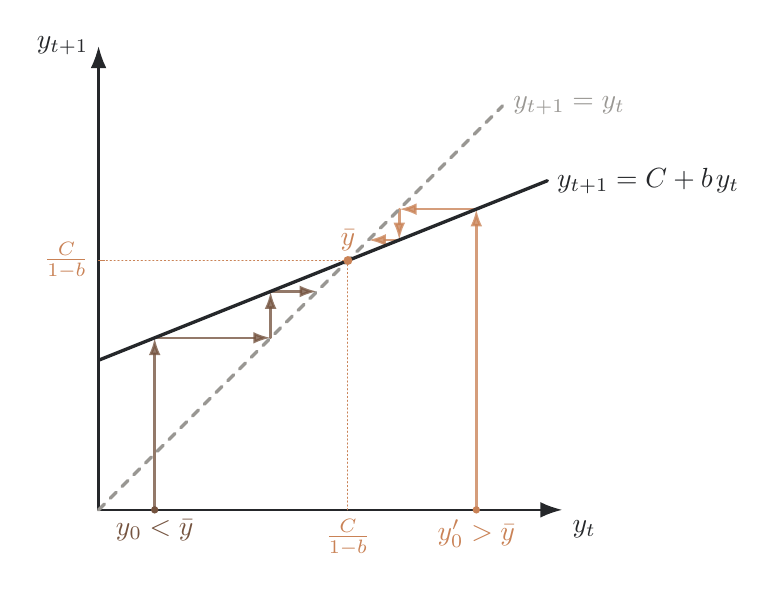
\begin{tikzpicture}[
        scale=0.95,
        line cap=round,
        line join=round,
        >=Latex,
        declare function={f(\x)=\C+\b*\x;}
    ]
        % Model parameters for y_t = C + b y_{t-1}
        \pgfmathsetmacro{\C}{2}
        \pgfmathsetmacro{\b}{0.40}
        \pgfmathsetmacro{\xmin}{0}
        \pgfmathsetmacro{\xmax}{6.2}
        \pgfmathsetmacro{\ymax}{6.2}
        \pgfmathsetmacro{\ybar}{\C/(1-\b)}

        % Initial x-axis positions for cobweb (one above and one below steady state)
        \pgfmathsetmacro{\xHi}{5.05}
        \pgfmathsetmacro{\xLo}{0.75}

        % Axes
        \draw[-{Latex[length=2.8mm,width=2mm]}, thick] (0,0) -- (\xmax,0) node[below right] {\(y_t\)};
        \draw[-{Latex[length=2.8mm,width=2mm]}, thick] (0,0) -- (0,\ymax) node[left] {\(y\nt\)};

        % Cobweb paths first (so they stay below the two main lines)
        \pgfmathsetmacro{\xk}{\xHi}
        \fill[DiagramHighlight] (\xk,0) circle (1.4pt);
        \node[DiagramHighlight, below] at (\xk,0) {\(y_0'>\bar y\)};
        \pgfmathsetmacro{\yk}{f(\xk)}
        \draw[-{Latex[length=2.2mm,width=1.5mm]}, DiagramHighlight, line width=0.9pt, opacity=0.78] (\xk,0) -- (\xk,\yk);
        \draw[-{Latex[length=2.2mm,width=1.5mm]}, DiagramHighlight, line width=0.9pt, opacity=0.78] (\xk,\yk) -- (\yk,\yk);
        \xdef\xk{\yk}
        \foreach \k in {2,...,2} {
            \pgfmathsetmacro{\yk}{f(\xk)}
            \draw[-{Latex[length=2.2mm,width=1.5mm]}, DiagramHighlight, line width=0.9pt, opacity=0.78] (\xk,\xk) -- (\xk,\yk);
            \draw[-{Latex[length=2.2mm,width=1.5mm]}, DiagramHighlight, line width=0.9pt, opacity=0.78] (\xk,\yk) -- (\yk,\yk);
            \xdef\xk{\yk}
        }

        \pgfmathsetmacro{\xk}{\xLo}
        \fill[DiagramComparison] (\xk,0) circle (1.4pt);
        \node[DiagramComparison, below] at (\xk,0) {\(y_0<\bar y\)};
        \pgfmathsetmacro{\yk}{f(\xk)}
        \draw[-{Latex[length=2.2mm,width=1.5mm]}, DiagramComparison, line width=0.9pt, opacity=0.78] (\xk,0) -- (\xk,\yk);
        \draw[-{Latex[length=2.2mm,width=1.5mm]}, DiagramComparison, line width=0.9pt, opacity=0.78] (\xk,\yk) -- (\yk,\yk);
        \xdef\xk{\yk}
        \foreach \k in {2,...,2} {
            \pgfmathsetmacro{\yk}{f(\xk)}
            \draw[-{Latex[length=2.2mm,width=1.5mm]}, DiagramComparison, line width=0.9pt, opacity=0.78] (\xk,\xk) -- (\xk,\yk);
            \draw[-{Latex[length=2.2mm,width=1.5mm]}, DiagramComparison, line width=0.9pt, opacity=0.78] (\xk,\yk) -- (\yk,\yk);
            \xdef\xk{\yk}
        }

        % Main lines on top
        \draw[dashed, DiagramGuide, very thick] (\xmin,\xmin) -- (5.4,5.4)
            node[pos=1, right] {\(y\nt=y_t\)};
        \draw[very thick, DiagramPrimary, domain=\xmin:6.0, samples=2]
            plot (\x, {f(\x)});
        \node[DiagramPrimary, right] at (6.0,{f(6.0)}) {\(y\nt=C+b\,y_t\)};

        % Fixed point marker
        \fill[DiagramHighlight] (\ybar,\ybar) circle (1.7pt);
        \draw[densely dotted, DiagramHighlight] (\ybar,0) -- (\ybar,\ybar);
        \draw[densely dotted, DiagramHighlight] (0,\ybar) -- (\ybar,\ybar);
        \draw[DiagramHighlight] (0,\ybar) -- (0.08,\ybar);
        \node[DiagramHighlight, left] at (0,\ybar) {\(\frac C{1-b}\)};
        \node[DiagramHighlight, below] at (\ybar,0) {\(\frac C{1-b}\)};
        \node[DiagramHighlight, above] at (\ybar,\ybar) {\(\bar y\)};
    \end{tikzpicture}
    \caption{\(0<b<1\) 情况下 \(\bkd{y_t}\) 的迭代图}
\end{figure}

作图的关键在于：在横轴确定 \(y_0\) 的位置，然后垂直向上到 \(f\bka{y_t}\) 曲线，意味着我们找到了 \(y_1\)；再水平到 45° 线，则是找到 \(y_1\) 在横轴上的位置，准备进入下一轮的迭代，去 \(f\bka{y_t}\) 上寻找 \(y_2\)。我们看到，无论初始值大于还是小于稳态，最终都会收敛到稳态 —— 系统的收敛性与初始位置无关。

最后来看参数 \(A\) 对收敛的影响。从差分方程的解 \ref{eq:DiffEquA} 可以看出 \(A=y_0-\bar y\)，即 \(A\) 是系统初始位置相对稳态的偏离。图中两条对比收敛轨迹刻画了不同 \(A\) 的情况，对比它们的水平线长度，发现：\(A\) 越大，即初始位置越远离稳态，每轮收敛的幅度就越大。

参数 \(A\) 由 \(C\) 和 \(b\) 构成，实际上，影响收敛速度的只有 \(b\)。为得到该结论，我们要观察 \(y\nt=f\bka{y_t}\) 直线和 45° 线的夹角：\(b\) 越大，夹角越大，收敛速度越快；反之收敛速度越慢。而 \(C\) \sidenote{注意 \sidemath{\(C\)} 值会影响 \sidemath{\(A\)}，所以 \sidemath{\(C\)} 不影响收敛速度但影响收敛时间}是使 \(y\nt=f\bka{y_t}\) 直线上下平移的参数，并不影响夹角的大小，因此不影响收敛速度。

\subsection{高阶差分系统的稳定性}{\label{subsec:HDiffSysStable}}

高阶系统难以作图，所以我们通过特征根来分析系统的稳定性\sidenote{一阶系统中 \sidemath{\(\lambda=b\)}，分析 \sidemath{\(b\)} 就是分析 \sidemath{\(\lambda\)}}。

\TopicLabel{初探稳定性}

接下来，解二阶线性差分系统
\begin{equation*}
    y\nnt + a_1\,y\nt + a_2\,y_t = C
\end{equation*}
写出特征方程
\begin{equation*}
    \lambda^2 + a_1\,\lambda + a_2 = 0
\end{equation*}
这是二次方程，特征根可能出现两实根、重根、共轭复根三种情况（由判别式 \(\Delta\) 可知）。我们用特征根表示系统的解，解如何得到略过
\begin{equation*}
    y^c=\begin{cases}
        \ A_1\,b^t_1+A_2\,b^t_2 & \n{ if}\quad \Delta>0\\
        \ A_3\,b^t + A_4\,t\,b^t & \n{ if}\quad \Delta=0\\
        \ \varrho^t\bks{A_5\,\cos\bka{t\,\theta} + A_6\,\sin\bka{t\,\theta}} & \n{ if}\quad \Delta<0
    \end{cases}
\end{equation*}
在复根的情况中，\(\varrho\) 是复根的模，\(\theta\) 是复根的辐角。

二阶线性差分系统稳定的条件是：
\begin{itemize}
    \item 当 \(\Delta>0\) 时，\(\bkf{\lambda_1}<1\) 且 \(\bkf{\lambda_2}<1\)
    \item 当 \(\Delta=0\) 时，\(\bkf{\lambda_{1,2}}<1\)
    \item 当 \(\Delta<0\) 时，\(\varrho<1\)（经计算得 \(\varrho=\dsq{a_2}\)）
\end{itemize}
我们在\ref{subsec:HDiffEqu} 中，我们把高阶线性差分系统转成由多个差分方程组成的一阶线性差分系统，可见无论几阶，线性差分系统的稳定性条件是相似的。这为我们的结论提供直觉，具体的证明略去。

\TopicLabel{深入稳定性}

判断稳定性最根本的方法是求解变量路径的表达式，计算它的极限查看是否收敛到固定值。求解路径是复杂的，所以在上一部分，我们简化到利用特征值就能判断稳定性。但其实还有更方便的方法：连特征值都不需要求出，只根据几个性质就能判断，这是我们即将要展开讨论的内容。

二阶线性系统的记特征多项式为
\begin{equation*}
    p\bka\lambda=\bkf{\bsA-\lambda\,\bsI}=\lambda^2 + a_1\,\lambda + a_2
\end{equation*}
则特征方程可表示为
\begin{align*}
    p\bka\lambda=\bka{\lambda-\lambda_1}\bka{\lambda-\lambda_2}= \lambda^2 - \bka{\lambda_1+\lambda_2}\lambda + \lambda_1\,\lambda_2=0
\end{align*}
根据线性代数的知识，该特征方程的一次项系数为矩阵 \(\bsA\) 的迹，常数项为矩阵 \(\bsA\) 的行列式。具体来说\sidenote{本笔记的 \sidemath{\(\bsA\)} 定义和课堂上的不同，相当于课堂上的 \sidemath{\(-\bsA\)}，所以计算出行列式相同但迹的符号相反}
\begin{align*}
    &T\coloneq \tr\bka{\bsA}=\lambda_1+\lambda_2=a_1\\
    &D\coloneq \det\bka{\bsA}=\lambda_1\,\lambda_2=a_2
\end{align*}

接下来，我们在不计算特征值的情况下，仅利用 \(T\) 和 \(D\) 对稳定性进行分析。对 \(\bka{T,D}\) 平面进行划分，划分依据有：
\begin{itemize}
    \item \(\Delta=0\) 抛物线：\(\Delta=T^2-4\,D\) 的符号决定特征根的类型
    \item \(D=1\) 水平线：稳定性要求两根的模都小于 1，必有 \(D=\lambda_1\,\lambda_2<1\)
    \item \(p\bka{1}=0\) 和 \(p\bka{-1}=0\) 斜线：这两条线分别对应某个特征根等于 \(1\) 或 \(-1\)，即特征根落在单位圆边界上。以 \(p\bka{1}\) 为例，考虑以下不等式
    \begin{align*}
        p\bka 1=\bka{1-\lambda_1}\bka{1-\lambda_2}<0
    \end{align*}
    在实根情形下，\(1-\lambda_1\) 与 \(1-\lambda_2\) 异号，说明两个特征根分别位于 \(\lambda=1\) 的两侧，因此至少存在一根满足 \(\lambda>1\)，系统不稳定。反过来，若 \(p\bka 1>0\)，两根同时大于或小于 1，仍然有可能发散，但其中存在稳定的可能。因此 \(p\bka{1}=0\) 和 \(p\bka{-1}=0\) 是重要边界。
\end{itemize}
从以上的说明我们已知 \(p\bka{1}=0\) 和 \(p\bka{-1}=0\) 对找到稳定区域重要，但不够充分，需配合 \(D=1\) 线一起使用。最终，我们可以得出稳定区域的边界由 \(D=1\)、\(p\bka{1}=0\)、\(p\bka{-1}=0\) 三条线构成，判别式只影响根的类型和系统运动的方式。

% 待完成：D 其实是 p(0)

\begin{figure}[H]
    \centering
    \sidenote{落在边界上也是不可能稳定的（排除特殊情况）；箭头表示大于的方向，如 \sidemath{\(p\bka{1}>1\)}}
    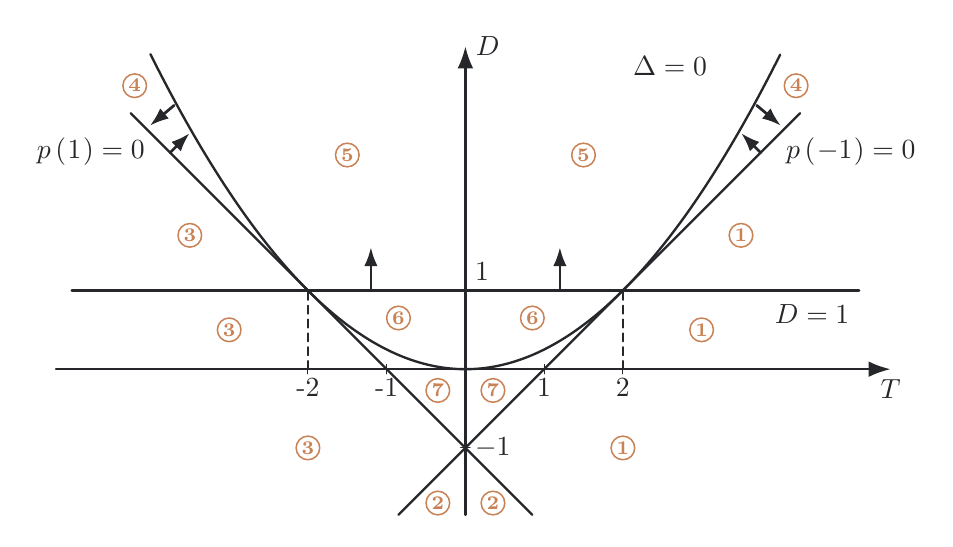
\begin{tikzpicture}[
        scale=1.0,
        line cap=round,
        line join=round,
        >=Latex
    ]
        % ---- User-tunable geometry ----
        \def\xmin{-5.2}
        \def\xmax{5.4}
        \def\ymin{-1.85}
        \def\ymax{4.1}
        \def\parabL{-4.00}
        \def\parabR{4.00}
        \def\lineL{-4.25}
        \def\lineR{4.25}
        \def\BaseLineWidth{0.85pt}
        \def\GuideLineWidth{0.60pt}
        
        \def\MirrorArrowLineWidth{1.00pt}
        \def\MirrorArrowALength{0.40}
        \def\MirrorArrowBLength{0.35}
        \def\MirrorArrowCLength{0.55}
        \def\MirrorArrowAY{3.35}
        \def\MirrorArrowBY{2.75}
        \def\MirrorArrowCY{1.00}
        \def\MirrorArrowAHalfGap{3.70}
        \def\MirrorArrowBHalfGap{3.75}
        \def\MirrorArrowCHalfGap{1.20}
        \def\MirrorArrowAAngle{-40}
        \def\MirrorArrowBAngle{135}
        \def\MirrorArrowCAngle{90}

        % ---- User-tunable label positions ----
        \def\pOneLabelX{-3.95}     \def\pOneLabelY{2.76}
        \def\pMinusOneLabelX{3.95} \def\pMinusOneLabelY{2.76}
        \def\DeltaLabelX{2.60}     \def\DeltaLabelY{3.85}
        \def\DOneLabelX{5.00}     \def\DOneLabelY{0.70}

        \def\labOneX{2.00}   \def\labOneY{-1.00}
        \def\labThreeX{-2.00}\def\labThreeY{-1.00}
        \def\labOneXX{3.00}   \def\labOneYY{0.50}
        \def\labThreeXX{-3.00}\def\labThreeYY{0.50}
        \def\labOneXXX{3.50}   \def\labOneYYY{1.70}
        \def\labThreeXXX{-3.50}\def\labThreeYYY{1.70}

        \def\labTwoX{0.35}   \def\labTwoY{-1.70}
        \def\labFiveX{1.50}  \def\labFiveY{2.72}
        \def\labSixX{0.85}   \def\labSixY{0.65}
        \def\labSevenX{0.35}\def\labSevenY{-0.27}

        \def\labFourX{4.20} \def\labFourY{3.60}

        \pgfmathsetmacro{\xcutL}{\ymin+1}
        \pgfmathsetmacro{\xcutR}{-1-\ymin}
        \pgfmathsetmacro{\MirrorArrowADx}{\MirrorArrowALength*cos(\MirrorArrowAAngle)}
        \pgfmathsetmacro{\MirrorArrowADy}{\MirrorArrowALength*sin(\MirrorArrowAAngle)}
        \pgfmathsetmacro{\MirrorArrowBDx}{\MirrorArrowBLength*cos(\MirrorArrowBAngle)}
        \pgfmathsetmacro{\MirrorArrowBDy}{\MirrorArrowBLength*sin(\MirrorArrowBAngle)}
        \pgfmathsetmacro{\MirrorArrowCDx}{\MirrorArrowCLength*cos(\MirrorArrowCAngle)}
        \pgfmathsetmacro{\MirrorArrowCDy}{\MirrorArrowCLength*sin(\MirrorArrowCAngle)}

        % Axes
        \draw[-{Latex[length=2.8mm,width=2mm]}, line width=\BaseLineWidth] (\xmin,0) -- (\xmax,0) node[below] {\(T\)};
        \draw[-{Latex[length=2.8mm,width=2mm]}, line width=\BaseLineWidth] (0,\ymin) -- (0,\ymax) node[right] {\(D\)};

        % Reference lines
        \draw[line width=\BaseLineWidth, DiagramPrimary] (\lineL,{-\lineL-1}) -- (\xcutR,\ymin);
        \draw[line width=\BaseLineWidth, DiagramPrimary] (\xcutL,\ymin) -- (\lineR,{\lineR-1});
        \draw[DiagramPrimary, line width=\BaseLineWidth] (-5,1) -- (5,1);
        \draw[DiagramPrimary, line width=\BaseLineWidth, domain=\parabL:\parabR, samples=320] plot (\x, {(\x*\x)/4});

        % Tick marks and labels
        \foreach \x/\lab in {-2/-2,-1/-1,1/1,2/2} {
            \draw (\x,0.06) -- (\x,-0.06);
            \node[below] at (\x,0) {\lab};
        }
        \draw (0.06,-1) -- (-0.06,-1);
        \node[right] at (0,-1) {\(-1\)};
        \draw (0.06,1) -- (-0.06,1);
        \node[above right] at (0,1) {\(1\)};

        % Helper guides at T = ±2
        \draw[DiagramPrimary, densely dashed, line width=\GuideLineWidth] (-2,0) -- (-2,1);
        \draw[DiagramPrimary, densely dashed, line width=\GuideLineWidth] (2,0) -- (2,1);

        % Labels for loci
        \node[DiagramPrimary, anchor=west] at (\pMinusOneLabelX,\pMinusOneLabelY) {\(p\bka{-1}=0\)};
        \node[DiagramPrimary, anchor=east] at (\pOneLabelX,\pOneLabelY) {\(p\bka{1}=0\)};
        \node[DiagramPrimary] at (\DeltaLabelX,\DeltaLabelY) {\(\Delta=0\)};
        \node[DiagramPrimary, left] at (\DOneLabelX,\DOneLabelY) {\(D=1\)};

        % Circled region numbers
        \newcommand{\RegionMarker}[4]{%
            \draw[color=#4, line width=0.55pt] (#1,#2) circle (0.15);
            \node[text=#4, font=\scriptsize\bfseries] at (#1,#2) {#3};
        }
        \RegionMarker{\labOneX}{\labOneY}{1}{DiagramHighlight}
        \RegionMarker{\labTwoX}{\labTwoY}{2}{DiagramHighlight}
        \RegionMarker{-\labTwoX}{\labTwoY}{2}{DiagramHighlight}
        \RegionMarker{\labThreeX}{\labThreeY}{3}{DiagramHighlight}
        \RegionMarker{\labFourX}{\labFourY}{4}{DiagramHighlight}
        \RegionMarker{\labFiveX}{\labFiveY}{5}{DiagramHighlight}
        \RegionMarker{\labSixX}{\labSixY}{6}{DiagramHighlight}
        \RegionMarker{\labSevenX}{\labSevenY}{7}{DiagramHighlight}
        \RegionMarker{-\labFiveX}{\labFiveY}{5}{DiagramHighlight}
        \RegionMarker{-\labSixX}{\labSixY}{6}{DiagramHighlight}
        \RegionMarker{-\labSevenX}{\labSevenY}{7}{DiagramHighlight}
        \RegionMarker{-\labFourX}{\labFourY}{4}{DiagramHighlight}
        \RegionMarker{\labOneXX}{\labOneYY}{1}{DiagramHighlight}
        \RegionMarker{\labThreeXX}{\labThreeYY}{3}{DiagramHighlight}
        \RegionMarker{\labOneXXX}{\labOneYYY}{1}{DiagramHighlight}
        \RegionMarker{\labThreeXXX}{\labThreeYYY}{3}{DiagramHighlight}

        % User-tunable mirrored arrows
        \draw[-{Latex[length=2.4mm,width=1.7mm]}, DiagramPrimary, line width=\MirrorArrowLineWidth]
            (\MirrorArrowAHalfGap,\MirrorArrowAY)
            -- ({\MirrorArrowAHalfGap+\MirrorArrowADx},{\MirrorArrowAY+\MirrorArrowADy});
        \draw[-{Latex[length=2.4mm,width=1.7mm]}, DiagramPrimary, line width=\MirrorArrowLineWidth]
            (-\MirrorArrowAHalfGap,\MirrorArrowAY)
            -- ({-\MirrorArrowAHalfGap-\MirrorArrowADx},{\MirrorArrowAY+\MirrorArrowADy});
        \draw[-{Latex[length=2.4mm,width=1.7mm]}, DiagramPrimary, line width=\MirrorArrowLineWidth]
            (\MirrorArrowBHalfGap,\MirrorArrowBY)
            -- ({\MirrorArrowBHalfGap+\MirrorArrowBDx},{\MirrorArrowBY+\MirrorArrowBDy});
        \draw[-{Latex[length=2.4mm,width=1.7mm]}, DiagramPrimary, line width=\MirrorArrowLineWidth]
            (-\MirrorArrowBHalfGap,\MirrorArrowBY)
            -- ({-\MirrorArrowBHalfGap-\MirrorArrowBDx},{\MirrorArrowBY+\MirrorArrowBDy});
        \draw[-{Latex[length=2.4mm,width=1.7mm]}, DiagramPrimary, line width=\MirrorArrowLineWidth]
            (\MirrorArrowCHalfGap,\MirrorArrowCY)
            -- ({\MirrorArrowCHalfGap+\MirrorArrowCDx},{\MirrorArrowCY+\MirrorArrowCDy});
        \draw[-{Latex[length=2.4mm,width=1.7mm]}, DiagramPrimary, line width=\MirrorArrowLineWidth]
            (-\MirrorArrowCHalfGap,\MirrorArrowCY)
            -- ({-\MirrorArrowCHalfGap-\MirrorArrowCDx},{\MirrorArrowCY+\MirrorArrowCDy});
    \end{tikzpicture}
    \caption{\(\bka{T,D}\) 平面中的稳定性分类示意图}
    \label{fig:TDStabilityMap}
\end{figure}

% 从上小节\ref{subsec:FDiffSysStable} 我们看出，一个系统是否稳定，只关系到齐次方程中的参数。故我们依 \ref{eq:DiffEquMatrix} 写出高阶差分系统的齐次方程组
% \begin{equation}
%     \bsX\nt+\bsA\,\bsX_t=\bs 0 \label{eq:DiffEquMatrixHom}
% \end{equation}
% 齐次的差分析系统有 \term{奇点}{singularity}，\(\bar{\bsX}=\bka{0,0}\)；如果系统有稳态点，那么稳态点就是该奇点。代入特征向量 \(\bs X_t=\lambda^{t}\,\bs v\) 得
% \begin{equation}
%     \lambda^{-2}\,\bs v + \bsA\,\lambda^{-1}\,\bs v = \bka{\lambda\,\bs I + \bs A}\,\bs v = \bs 0
% \end{equation}
% 同样，特征值的实虚及其大小决定系统的稳定性。写出特征方程
% \begin{equation}
%     \det\bka{\lambda\,\bs I + \bs A} = \matbkf{a_1&a_2\\-1&0}+\matbkf{\lambda&0\\0&\lambda} = \matbkf{\lambda+a_1 & a_2\\-1 & \lambda} = \lambda^2 + a_1\,\lambda + a_2 = 0
% \end{equation}
% 该二次方程解的情况只与 \(a_1\) 和 \(a_2\) 值相关，它们分别是矩阵 \(\bsA\) 的迹（记 \(T\)）和行列式（记 \(D\)），那么高阶线性差分系统的稳定性转向对 \(T\) 和 \(D\)的分析。我们直接得出如下结论\footnote{参考《常微分方程》（丁同仁和李承治，2022）定理 8.5：初等奇点类型的判定}

\TopicLabel{奇点的分类}

我们分别假设特解的形式为 \(k_1\)、\(k_2\,t\) 和 \(k_3\,t^2\)，二阶线性差分方程的特解为 \footnote{2026 年 4 月 21 日勘误：此前第二种情况有误}
\begin{equation}
    y^p=\begin{cases}
       \ \dfrac C{1+a_1+a_2} & \n{ if}\quad 1+a_1+a_2\neq 0\\[2ex]
       \ \dfrac {C}{2+a_1}\cdot t & \n{ if}\quad 1+a_1+a_2=0\ \n{ and}\ a_1\ne-2\\[2ex]
       \ \dfrac {C}{2}\cdot t^2& \n{ if}\quad a_1=-2\ \n{ and}\ a_2=1
    \end{cases}
\end{equation}
称 \(y^p\) 称作 \term{奇点}{singularity}。奇点不一定是稳定点，但它对系统至关重要 —— 即使系统是发散的，系统也是围绕它运动。我们用下表总结奇点的类型以及判定条件。
\begin{table}[htbp]
    \centering
    \renewcommand{\arraystretch}{1.5}
    \begin{tabular}{>{\centering\arraybackslash}p{0.06\linewidth}>{\centering\arraybackslash}p{0.28\linewidth}>{\centering\arraybackslash}p{0.21\linewidth}>{\centering\arraybackslash}p{0.12\linewidth}>{\centering\arraybackslash}p{0.175\linewidth}}
        \toprule
        序号 & 条件 1 & 条件 2 & 类型 & 稳定\\
        \midrule
        1 & \(p\bka{1}<0\,, \ p\bka{-1}>0\) &  & 实鞍点 & 发散\\
        2 & \(p\bka{1}<0\,, \ p\bka{-1}<0\) &  & 实结点 & 发散\\
        3 & \(p\bka{1}>0\,, \ p\bka{-1}<0\) &  & 实鞍点 & 发散\sidenote{准确地说：当奇点为鞍点时，只存在两条收敛路径，其余发散}\\
        4 & \(p\bka{1}>0\,, \ p\bka{-1}>0\) & \(\Delta>0\,,\ D>1\) & 实结点 & 发散\\
        5 & \(p\bka{1}>0\,, \ p\bka{-1}>0\) & \(\Delta<0\,,\ D>1\) & 虚焦点 & 震荡发散\\
        \midrule
        6 & \(p\bka{1}>0\,, \ p\bka{-1}>0\) & \(\Delta<0\,,\ D<1\) & 虚焦点 & 震荡收敛\\
        7 & \(p\bka{1}>0\,, \ p\bka{-1}>0\) & \(\Delta>0\,,\ D<1\) & 实结点 & 多种收敛情况\sidenote{结合 \sidemath{\(\Delta\)} 与 \sidemath{\(D\)} 值可得 \sidemath{\(T\)} 的范围，而对区域 \sidemath{\(7\)} 做更细致的划分，此处省略；\sidemath{\(T\)} 的符号影响根的符号}\\
        \bottomrule
    \end{tabular}
    \caption{奇点类型与稳定性的判定表}
    \label{tab:SingularityClassification}
    \renewcommand{\arraystretch}{0}
\end{table}

\ref{fig:Sing} 以微分系统为例（因为差分系统是离散的，不便展示），汇总了各种稳定和不稳定奇点类型的图像 —— 强调曲线是序列随时间运动的轨线，辅助箭头是系统在每个位置的运动方向。

有几个不同的特征根，代表需要多少个基向量构成特征向量空间。以第二行图像为例：首先，它们都有两个不同实特征根，所以我们能在图像中找到两个垂直方向，它们足够代表整个系统的运动方向，并且如果走上了这两条路径，那么系统会沿直线运动。在 (e) 和 (f) 图中，我们不区分实根是否是异号；如果是异号，那么系统会在对称路径上来回跳跃，这较难用图像展示，但异号会导致震荡，这一特性仍然存在。

出现复根的系统必然震荡，这是因为 \(i^2=-1\) 相当于出现了负号\footnote{2026 年 4 月 19 日勘误：此前句中公式存在错误} 。(h) 图 \(\varrho=1\) 情况很好展示了系统在单位圆上 “震荡”（实际上是在复平面上旋转）的效果。

\begin{figure}[H]
    \MaybeIncludeGraphics[width=\linewidth]{chapter-07-singularity.png}
  \caption{各种奇点类型汇总图}
  \label{fig:Sing}
\end{figure}


%% ====================================================
%% 章内附录
%% ====================================================
\BeginChapterAppendix

\section{特征方程法}{\label{sec:CharEquMethod}}

定义位移算子 \(L\) 作用在 \(\bkd{x_t}\) 上的结果为 \(L\,x_t = x\lt\)；恒等算子 \(I\) 的效果为 \(I \, x_t=x_t\)。位移算子也有自己的特征值和特征向量，仿照线性变换的\sidenote{参考了线性变换的特征值和特征向量满足 \sidemath{\(\bs A\,\bs x=\lambda\,\bsx\)}}，写出
\begin{equation}
    L\,x_t=\lambda\,x_t=x\lt
\end{equation}
那么特征值为 \(\lambda\)；由 \(x_t=\lambda^{-1}\,x\lt=\lambda^{-2}\,x\llt\) 得特征向量为 \(x_t=C\,\lambda^{-t}\)（\(C\) 为任意常数），该特征向量正是我们求解齐次方程时 “猜测” 的解的结构。

为了更容易看出形式，我们对二阶线性齐次差分方程
\begin{equation}
    x_t + a_1\,x\lt + a_2\,x\llt=0
\end{equation}
展开讨论。改写差分方程得
\begin{align}
    x_t + a_1\,L\,x_t + a_2\,L^2\,x_t &= 0\notag\\
    x_t + a_1\,\lambda\,x_t + a_2\,\lambda^2\,x_t &= 0\notag\\
    1 + a_1\,\lambda + a_2\,\lambda^2 &= 0
\end{align}
这是由特征多项式（等式左侧）构成的\,\AccentTerm{特征方程}，其解为特征值。通过特征值找到对应的特征向量，再对不同特征值的特征向量进行线性组合得二阶线性差分方程的齐次解。

不失一般性地，求解线性齐次差分方程（无论几阶），实际上就是解特征方程。之所以能这么做，是得益于我们要解的差分方程具有线性性，齐次解族可以形成向量空间\sidenote{此处 “向量” 有更广泛的含义}；反之，若不具有线性性，往往会违背向量空间所要求的加法封闭性，无法形成向量空间。而要猜测齐次解形为 \(C\,\lambda^{-t}\)，一方面我们目前所考虑的线性差分方程满足所需形式，特征向量确为其解；另一方面特征向量凝聚了位移算子的性质，是最具代表性的，也是最容易捕获的。

\section{复合增长}\label{sec:CompGrow}

假设某国 GDP 的增长率保持在 5\%。GDP 是典型的复合增长变量，即经济总是在过往的基础上增长的，过去的发展成果不会凭空消失。那么过去 \(t\) 年后，该国的 GDP 将达到
\begin{equation*}
    Y_t = Y_0 \cdot \bka{1+0.05}\cdot  \cdots\cdot \bka{1+0.05}=Y_0 \cdot 1.05^t\notag
\end{equation*}
将其取对数得
\begin{equation}
    \log Y_t=Y_0 \cdot t\cdot\log 1.05\sim C\cdot t \label{eq:CompGrowLog}
\end{equation}
可见我们只有做对数运算，对数变量才会呈现出线性的增长趋势，符合我们在求解线性差分方程中所假设的特解形式。

如果我们把复合增长压榨到极值，会发生什么结果？考虑一年内有 \(n\) 个单位时间，增长率 \(g\) 被平均分成 \(n\) 份，得到每个单位时间的增长率，再进行复合增长，得到
\begin{align}
    Y_1 &= Y_0 \cdot \bka{1+\frac{g}{n}} \cdot \dots \cdot \bka{1+\frac{g}{n}}= Y_0 \cdot \bka{1+\frac{g}{n}}^n\to Y_0 \cdot \n e^{g}\,, \quad \nti\notag
\end{align}
以上只计算了一年内的连续增长，若计算 \(t\) 年内的连续增长，则 \(Y_t=Y_0 \cdot \n e^{g\,t}\)，我们称其中 \(g\) 为\,\AccentTerm{连续增长率}\,或\,\AccentTerm{瞬时增长率}。解 \(\n e^g=1.05\)，不难得到以 \(g=\log 1.05\) 的连续增长率增长，即可实现 5\% 的年增长率。

连续增长率 \(g\) 与年增长率 \(g'\) 的关系为
\begin{equation}
    g' = \n e^g - 1 \quad \Leftrightarrow \quad g = \log\bka{1+g'}
\end{equation}
当 \(g'\) 很小时，\(g'=\n e^g-1\approx g\)，连续增长率和年增长率几乎没有区别；当 \(g'\) 较大时，\(g\) 会明显小于 \(g'\)，连续增长率和年增长率的差异就比较大。

以上计算的都是都是一年内的连续增长，如果时间长到 \(t\) 年内的连续增长，则 \(Y_t=Y_0 \cdot \n e^{g\,t}\)。我们对该结果取对数得
\begin{align}
    \log Y_t=Y_0 + g\,t \notag
\end{align}
有趣的事情发生了：若要实现 5\% 的年增长率目标，\(g=\log1.05\)，此时该结果就是 \ref{eq:CompGrowLog} 中的结果。所以，复合增长的变量服从指数增长，取对数可以剥离出连续增长率。

%% ====================================================
%% 章内参考文献
%% ====================================================
% \PrintChapterBibliography

\FinishStandaloneChapter
